\documentclass[10pt]{article}

\usepackage[margin=1in, bottom=0.9in]{geometry}

\setlength{\parindent}{0pt}

\usepackage{listings}
\lstset{
    language=R,
    language=SQL, 
    basicstyle=\ttfamily
}
\usepackage{biblatex}
\usepackage{subcaption} 
\usepackage{mlmodern}
\usepackage[section]{placeins}
\usepackage{xcolor}
\usepackage[]{amsthm}
\usepackage[]{amsmath}
\usepackage[]{amsfonts}
\usepackage{bm}
\usepackage{graphicx}
\usepackage{makecell}
\usepackage{booktabs}
\usepackage{rotating}
\usepackage{multirow}
\graphicspath{ {./Images/} }
\addbibresource{Fc_StackEx_Counts_Paper.bib}
\DeclareMathOperator*{\argmin}{argmin} 

\newtheorem{theorem}{Theorem}
\newtheorem{corollary}{Corollary}[theorem] % Use theorem counter as `parent`
\newtheorem{lemma}{Lemma}


\definecolor{codegreen}{rgb}{0,0.6,0}
\definecolor{codegray}{rgb}{0.5,0.5,0.5}
\definecolor{codepurple}{rgb}{0.58,0,0.82}
\definecolor{backcolour}{rgb}{0.95,0.95,0.92}

\lstdefinestyle{mystyle}{
    backgroundcolor=\color{white},   
    commentstyle=\color{codegreen},
    keywordstyle=\color{magenta},
    numberstyle=\tiny\color{codegray},
    stringstyle=\color{codepurple},
    basicstyle=\ttfamily\footnotesize,
    breakatwhitespace=false,         
    breaklines=true,                 
    captionpos=b,                    
    keepspaces=true,                 
    numbers=left,                    
    numbersep=5pt,                  
    showspaces=false,                
    showstringspaces=false,
    showtabs=false,                  
    tabsize=2
}

\lstset{style=mystyle}


\title{\vspace{-2.0cm}Final Project | Forecasting Monthly ``Time-Series'' Related Questions on the Stack Exchange}
\author{Andrew Mashhadi}
\date{Spring 2023}

\begin{document}

\maketitle

\section*{Introduction} 

Since 2008, the \textit{Stack Exchange} has been one of the most popular networks of question-and-answer websites. The Stack Exchange network consists of over 100 different websites, covering a variety of specific topics and subjects. As of today, the most actively used sites within the Stack Exchange network are Stack Overflow, which consists of computer programming questions, and Mathematics, which consists of mathematics related questions. Questions asked on these websites are usually technical, and are generally about the details of a specific subject under the given category of the Stack Exchange website. The question-and-answer platform can often be an excellent resource for users looking to learn more about very specific topics that may arise during an academic course, at work, or while self-studying. When submitting a question, each Stack Exchange website offers an option to use tags to help other users find the questions they may be interested in answering, and to help future users find questions they may also have. The number of questions with specific tags over time may serve as a useful dataset to researchers looking to characterize the interest of certain topics over time.

\

\textit{Time series analysis} is a topic within mathematics and statistics that encompasses techniques for examining or modeling data points arranged in chronological order, with the aim of extracting meaningful statistics and other characteristics from the data. While traditional time series analysis has a long history spanning several decades, the recent surge in machine learning and data science has sparked a renewed interest in this subject. This course, \textit{Stats 415}, also happens to focus primarily on time series analysis and its applications. Therefore, in this study, we aim to analyze and model the monthly count of Stack Exchange questions tagged with ``time-series'', using a variety of methods and approaches discussed in class. In addition, we would like to use our final model to provide a forecast of the monthly counts of ``time-series'' related questions asked over the next few years. 


\section*{Data}

As mentioned in the previous section, our data will consist of monthly counts of Stack Exchange questions tagged with ``time-series''. In other words, the data will be the number of time series related questions for each available month. Fortunately, the Stack Exchange provides an open source tool known as the \textit{Stack Exchange Data Explorer} for running arbitrary SQL queries against public data from the Stack Exchange network \cite{stex_de}. This tool includes collaborative query editing for all graduate and public Stack Exchange websites. The SQL query used for this paper is provided in the Appendix.

\

The Stack Exchange Data Explorer was used to collect and save all available ``time-series'' tagged questions. The data consisted of monthly counts from January 2009 to May 2023, with no missing entries. Therefore, our full data set contained exactly $n=173$ observations. The first 90\% of our dataset (Jan. 2009 - Nov. 2021) was used as a designated training set and the remaining 10\% (Dec. 2021 - May 2023) was used as an ``unseen'' testing set. We display the monthly counts of ``time-series'' tagged questions from our training set in Figure (1). We immediately notice that there is a clear upward trend in the data from 2009 to 2021. This may be due to the increasing interest in time series analysis, however, it could also be due to other factors such as an increase of users on the Stack Exchange network. Additionally, we notice the obvious spike in counts occurring in 2020. This relatively large spike is most likely a result of the COVID-19 pandemic. Time series analysis and modeling were often used to predict or forecast surges in cases or deaths throughout the pandemic.

\

We also assess the \textit{autocorrelation} (ACF) and the \textit{partial autocorrelation} (PACF) for the raw counts in our training data. The plots shown in Figure (2) indicate that the trend and/or cycles in our data need to be removed before we begin modeling. In particular, we can see from the large ACF values displayed in the top plot of Figure (2) that our data is currently being dominated by the trend. The ACF is larger than the upper bound of the confidence band for the first 20 lag values. Assuming our data is trend stationary, the strong trend in our data will most likely obscure the behavior of the associated stationary process and prevent us from successfully fitting any \textit{autoregressive moving average} (ARMA) models. The strong trend would also introduce extremely low frequency components in a periodogram that may obscure the appearance at higher frequencies and would most likely prevent us from accurately performing a spectral analysis.

\section*{Removing Trend}
 
If we assume our model is trend stationary, our original observations, $x_t$, are composed of a trend, $\mu_t$, and a stationary process, $y_t$, such that:

$$ x_t = \mu_t + y_t$$

for $t = 1, 2, ..., 173$. As discussed at the end of the previous section, the trend, $\mu_t$, must be removed before we can conduct much of our analysis and modeling. In this section, we discuss the steps involved to obtain a reasonable estimate of the trend component, $\hat \mu_t$, and then work with the corresponding residuals

$$\hat y_t = x_t - \hat \mu_t$$

in our remaining analysis and modeling sections.

\

From Figure (1), we can see that the relationship between the time and the monthly counts does appear non-linear, but a linear fit may be able capture the majority of the trend. Therefore, we first fit the training data using linear regression, and then we fit the training data with a third-order polynomial. Using an ANOVA table, we rejected the hypothesis that the linear fit was sufficient, and found that the third-order polynomial had a significantly better fit of the data (see Table (1)). That is, we found that the drop in the RSS was effectively ``worth'' the cost of two additional degrees of freedom. The polynomial fit's F-test resulted in a p-value close to 0, and the R-Squared was approximately 0.92, suggesting that the third-order polynomial fits the training data very well and is able to explain a large proportion of the variance (see Table (2)). Visually, we can see the third-order polynomial was successfully fit to the training data in Figure (3). Therefore, using the computed coefficients from the polynomial fit, our final estimate of the trend is:

$$\hat \mu_t = 78.95 + 651.301t - 16.89t^2 - 66.86t^3$$

Now that we have found an acceptable fit for our trend, we subtract our fitted values, $\hat \mu_t$, from the raw counts, $x_t$, to obtain our detrended residuals, $\hat y_t$. We can see from Figure (4) that the detrended residuals, $\hat y_t$, resembles the stationary time series that we desire.

\section*{Spectral Analysis}

Now that we have successfully removed the trend from our training data, we investigate the fluctuations in the detrended counts in search of obvious cycles. To do this, we estimate the spectrum of our detrended training data to help us determine predominant periods and to obtain confidence intervals for the identified periods. In Figure (5), we display the periodogram without smoothing (top) and the periodogram with nonparametric smoothing (bottom). The \textit{modified Daniell kernel} with $L=5$ and a 20\% taper was used for the nonparameteric smoothing method. In addition, we separately fit the parametric (autoregressive) spectral estimator shown in the bottom of Figure (6). To fit the autoregressive spectral estimator, we found the AR model that minimized the training \textit{root mean squared error} (RMSE). We can see from the top plot of Figure (6) that the AR(15) model minimized the training RMSE, so we believe it provided the best fit AR model. Therefore, the spectrum of the fitted AR(15) model was used to provide the parametric spectral estimator.

\

From all three spectral estimators shown in Figures (5) \& (6), the frequency axis is in cycles per year (in this case, $\texttt{frequency} * 12$, because data points were taken monthly). Additionally, all three spectral estimations illustrate an obvious peak at $\omega \approx 1\cdot\frac{1}{12}=\frac{1}{12}$ (1 year), along with two other potentially significant peaks at $\omega \approx \frac{3}{10}\cdot\frac{1}{12}=\frac{1}{40}$ (40 months) and $\omega \approx 3\cdot\frac{1}{12}=\frac{1}{4}$ (4 months). Using the periodogram with nonparametric smoothing, we generated the approximate one-sided and two-sided 95\% confidence intervals for the true spectral power at the three frequencies of interest (shown in Table (3)).

\

In all spectral estimates, the narrow peak at frequency $w \approx \frac{1}{12}$ achieves the highest estimated spectral power and represents the annual cyclical pattern clearly displayed in the detrended residuals (Figure (4)). Since the lower bound of the one-sided confidence interval shown in Table (3) is much larger than all other (near-by) periodogram ordinates, we have evidence suggesting that the frequency $\omega \approx \frac{1}{12}$ (1 year) corresponds to a statistically significant peak. This apparent annual cycle may be from academic institutions teaching ``time-series'' courses during select terms of the school year, leading to more or less questions posted online depending on the time of year. In Figure (7), we illustrate the cyclical behavior occurring in each year by stacking the plots of the detrended monthly counts from 2014, 2015, 2016, and 2017. The annual cycle seen in each plot may be described with the following stages: (1) an increase in values within the first quarter of the year (2) a drop in values between April, May, and June (3) higher values by August (the Summer) (4) extremely low values in September (5) an increase in values up to a relative peak in November and (6) values then drop in December (Winter break).

\

The peak at $\omega \approx \frac{1}{40}$ is also seen in all three spectral estimates. We can see from the spectral estimations in Figures (5) \& (6) and the associated confidence intervals from Table (3) that this peak has a much wider band and does not appear to have significantly large spectral power. The wider band typically suggests that this cycle may be slightly irregular. In fact, only looking at the two nonparameteric spectral estimations may lead us to believe that this 40-month cycle is simply due to random noise in our data. However, the parametric spectral estimation also displays a somewhat large spike in the neighborhood of $\omega \approx \frac{1}{40}$. Since parametric autoregressive spectral estimators generally have superior resolution in problems when several closely spaced narrow spectral peaks are present \cite{Shumway}, we believe there is a 40-month cycle in our data. 

\

All three spectral estimates also indicate another small peak at $\omega \approx \frac{1}{4}$. This peak seems to have a wider band than the peak associated with the annual cycle, but not as wide as the peak associated with the 40-month cycle. Although the absolute spectral power is not as large as the other two peaks, the lower bound of the one-sided confidence interval shown in Table (3) is also larger than all other (near-by) values. This indicates that the frequency $\omega \approx \frac{1}{4}$ corresponds to a statistically significant peak. The wider band associated with this peak also suggests that this cycle is irregular, but tends to be
around 4 months on average. Such a cycle may be from the general structure of time-series courses taught each academic term. For instance, we may see an increase of online posts when more advanced topics are reached in the later weeks of a typical time series analysis course. 

\

It is important to note that the frequency associated with the 4-month peak is located at a multiple of $\omega \approx \frac{1}{12}$, so it may simply be a \textit{harmonic} of the annual cycle seen earlier. Since we do not see a harmonic at $\omega \approx \frac{2}{12}$, we do not believe this is the case. However, this consideration was made before removing the cycle from our data.

\

After identifying the three predominant cycles in the detrended training data, we iteratively removed each of them from our data. For each cycle, we first averaged the remaining monthly residuals over the cycle's associated period, and then subtracted the averages from each corresponding data point. In Figures (8)-(10) we display each cycle's associated average values (top) and the residuals remaining after removing the cycle from the data (bottom). After all three observed cycles were effectively removed from the detrended data, we computed the ACF and PACF from our remaining, \textit{final}, residuals (Figure (11)). We see that the ACF and PACF values are no longer dominated by trend or seasonality, indicating that the data may now be appropriately used with our models.

\section*{Modeling}

Now that we have removed both trend and cycles from our training data, we proceed to fit our ARMA models. In each ARMA model, the order of the autoregressive (AR) and moving average (MA) processes are represented by $p$ and $q$, respectively. As depicted in Figure (11), the ACF and PACF values do not exhibit a definitive cutoff at a specific lag. This observation suggests that our final residual data may conform to an ARMA model (such that $p>0$ and $q>0$). To explore the potential success of different models comprehensively, we conduct a grid search to tune our ARMA model and identify the optimal parameters within the ranges of $p=0, 1, ..., 11$ and $q=0, 1, ..., 11$.

\

We evaluated a total of 144 ARMA($p$, $q$) models fit to the data, and calculated the \textit{Akaike Information Criterion} (AIC) for each model. The AIC served as a criterion to identify the optimal ARMA model by determining the combination of $p$ and $q$ that minimized the AIC. To visually compare the AIC values associated with each model, we generated Figure (12). By examining the plot, we observed that while a few other models displayed similar AIC scores, the ARMA(3, 8) model achieved the lowest AIC score of 1197.51 (represented by the red dot in Figure (12)). Consequently, we conclude that the ARMA(3, 8) model provides the best fit to the final residuals obtained from the training data. Using the estimated coefficients, the fitted ARMA(3, 8) model may be written in its complete mathematical form as follows:


\begin{align}
    \begin{split}
        r_t = {}& 0.107 - 0.407r_{t-1} + 0.470r_{t-2} + 0.631r_{t-3} + w_{t} + 0.763w_{t-1} - 0.279w_{t-2} \\
                &  - 0.754w_{t-3} - 0.060w_{t-4} + 0.030w_{t-5} - 0.073w_{t-6} - 0.334w_{t-7} - 0.311w_{t-8} \nonumber
    \end{split}
\end{align}

where $r_t$ represents our time series of interest (the final residuals) and $w_t \sim wn(0, \sigma_w^2)$. Notice from the equation that the value of the final residual at time $t$, $r_t$, is positively related with the values at $t-2$ and $t-3$, but it is negatively related to the previous value at $t-1$. That is, with all else being equal, large positive values observed 2 or 3 months in the past will generally lead to an increase in the predicted value for the current month, but a large positive value observed in the previous month will generally decrease the predicted value for the current month.

\

Subsequently, we proceeded to generate diagnostic plots for the residuals of our selected optimal model. These plots include the standardized residuals over time, the ACF of the residuals, a normal Q-Q plot of the standardized residuals, and the p-values associated with the Q-statistic (as depicted in Figure (13)). Upon analyzing the time plot of the standardized residuals, no discernible patterns were observed, and only a single outlier was seen surpassing 3 standard deviations in magnitude during 2020. The ACF plot of the standardized residuals displayed no significant deviations from the model assumptions, and the Q-statistic remained non-significant across the depicted lags. The normal Q-Q plot of the residuals indicated a reasonable adherence to the assumption of normality, albeit with a couple potential outliers. Additionally, we computed the spectrum of the residuals from our fitted ARMA(3, 8) model, as illustrated in Figure (14). We can see that there are no significantly large, or outlying, spikes within the estimated spectrum, suggesting that there are no obvious cycles remaining in our model's residuals. Therefore, we conclude that our ARMA(3, 8) model was able to successfully fit the detrended and cycle-removed data.

\section*{Predictions \& Forecasting}

Based on the residual analysis, the model appears to adequately fit the training data with trend and cycles removed. However, we also want to examine our model's overall fit of the original data, in raw counts of ``time-series'' questions. Furthermore, we would like to assess how well our model performs on the completely unseen test data. Therefore, we generated predictions from our ARMA(3, 8) model for both the training data and the testing data, then we added the associated trend and cycles back into these values to obtain our final predictions in units of monthly counts of ``time-series'' questions. We should note that the predictions associated with the test set were generated using an 18-step \textit{long-term forecast horizon}. That is, only the data from January 2009 to November 2021 was used to generate the predictions from December 2021 to May 2023 (the test data). Figure (15) displays the predictions (red) overlayed on the original monthly counts from the training and testing data (black). The shaded blue region beginning in 2021 represents the predictions corresponding to the unseen test data. Although the predictions generally seem to line up quite nicely with the true data, the predictions for the test data certainly appear to have a slightly larger error than the predictions for the training data. In fact, the RMSE for the testing data was found to be 23.25 counts, while the RMSE for the training data was found to be 10.34 counts. Considering that the number of the ``time-series'' questions are within the range of roughly 0-200 counts, these are both relatively good margins of error to achieve. Our model may be struggling to accurately predict the monthly counts due to the disruption that COVID-19 had on the interest in ``time-series'' related topics beginning in 2020. However, it is not uncommon for testing error to be larger than the training error. In general, the overall training and testing performances still indicate that our chosen model is demonstrating an excellent fit and good predictive power for future counts of ``time-series'' data.

\

To wrap up this section, we proceed to retrain our model using all available data and generate forecasts extending up to May 2026. Our decision to retrain the model with the testing data included was driven by the objective of maximizing data utilization and ensuring the model's up-to-dateness prior to forecasting. In this case, we used another long-term, 36-step, forecast horizon when generating our predictions. Figure (16) presents the raw counts (black), the fitted values (red), and the generated forecasts (blue), accompanied by the associated $\pm1$ standard error ($S.E.$) depicted by the gray shading. The forecasted trend indicates that the number of questions tagged as ``time-series'' will reach a plateau throughout 2023 and will follow by a gradual decline leading up to May 2026.


\section*{Conclusion}

In this paper, we conducted an analysis of monthly counts of Stack Exchange questions tagged with ``time-series'' using various methods and approaches discussed in the course. We started by obtaining the data from the Stack Exchange Data Explorer and preprocessing it by removing the trend. We then performed spectral analysis to identify obvious cycles in the detrended data, finding an annual cycle, a 40-month cycle, and a 4-month cycle. After removing these cycles, we obtained the final residuals and proceeded to fit autoregressive moving average (ARMA) models. Based on the Akaike Information Criterion (AIC), the ARMA(3, 8) model was selected as the best fit ARMA model. 

\


We assessed our fitted model's performance (with and without the cycles and trend included) using a variety of plots, diagnostics, tests, and performance metrics. The RMSE scores reported for the training and testing data were 10.34 counts and 23.25 counts, respectively. These scores, coupled with the generated figures discussed earlier, indicated an excellent fit of our model and reasonable predictive capability for future counts of ``time-series'' tagged questions. Moreover, we utilized our final model to forecast the monthly occurrence of ``time-series'' questions until May 2026. According to our 3-year forecast, the number of questions tagged with ``time-series'' will eventually reach a plateau within the next year and will then gradually decline until May 2026. Overall, our analysis provided insights into the time-dependent behavior of ``time-series'' tagged questions on the Stack Exchange and offers a forecasting model for future monthly counts.

\

Due to the monthly nature of our dataset and the relatively short existence of the Stack Exchange platform for approximately 15 years, our available data is limited to just $n=173$ observations, which may be considered insufficient by current standards. To enhance future studies, it would be beneficial to explore additional data sources with a longer time span or higher frequency of collection (e.g., daily or weekly). Moreover, it is evident that the COVID-19 pandemic had a clear impact on the monthly counts of ``time-series'' tagged questions in 2020, which seemingly influenced the subsequent years as well. Therefore, when sufficient time has passed, it would be advantageous to conduct a similar analysis specifically for the period \textit{after} 2020 in order to compare it with our existing model. Lastly, it should be noted that the slight downward trend observed in the previous section's forecasts may be attributed to the polynomial fit of the trend. Polynomial fits typically struggle with extrapolation, as they tend to diverge rapidly when extending beyond the observed time range. Hence, future work should also consider alternative methods for trend fitting to mitigate this limitation.

\newpage 

\printbibliography

\newpage

\section*{Appendix}

\subsection*{Figures}

\begin{figure}[ht!]
    \centering
    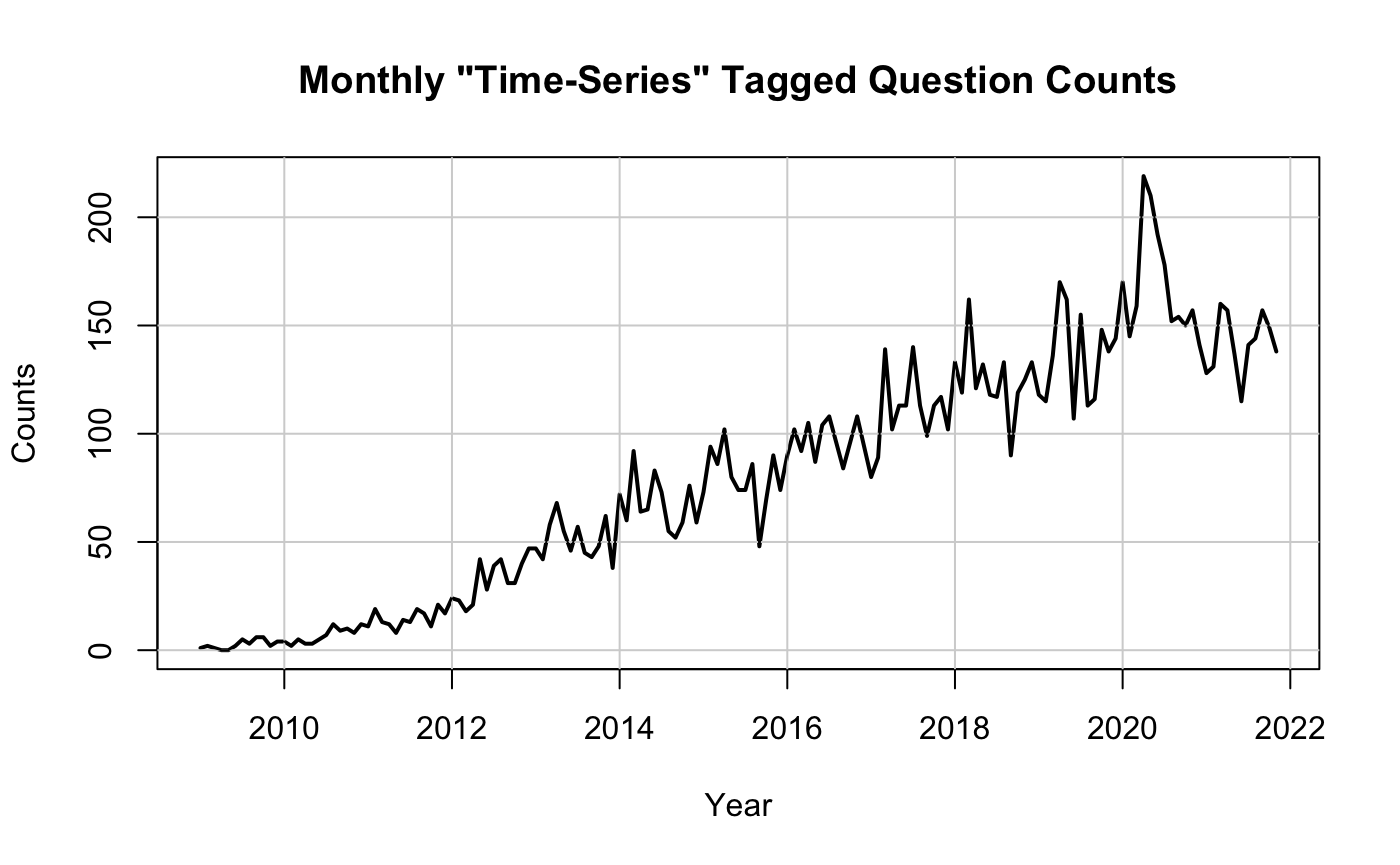
\includegraphics[height=85mm, width=115mm]{trn_raw_counts.png}
    \caption{Raw Counts From Training Data}
\end{figure}

\begin{figure}[ht!]
    \centering
    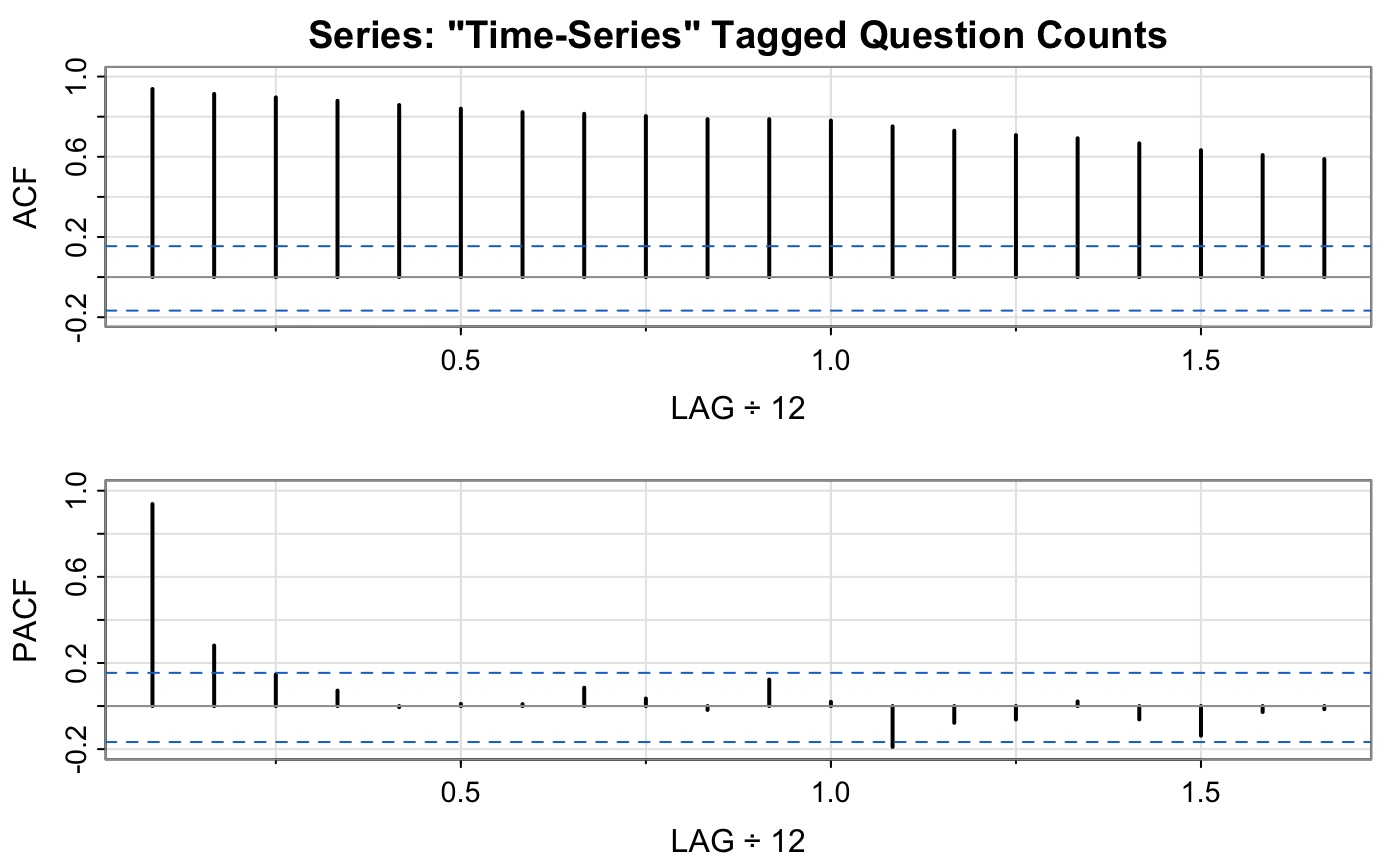
\includegraphics[height=85mm, width=115mm]{acf2_raw_counts.png}
    \caption{ACF and PACF for Raw Counts From Training Data}
\end{figure}

\begin{table}[h!]
    \centering
    \begin{tabular}{| c | c | c | c | c | c | c | } 
    \hline
    Fit & Resid. Df & RSS & DF & Sum. Sq. & $F$ & Pr($>F$) \\ 
    \hline
    \hline
    Linear Fit & 153 & 42070 & & & & \\
    \hline
    Poly Deg. 3 & 151 & 37315 & 2 & 4755.2 & 9.621  & $< 0.001$\\
    \hline  
    \end{tabular}
    \caption{Analysis of Variance Table}
\end{table}

\begin{table}[h!]
    \centering
    \begin{tabular}{| c | c | c | c | c |} 
    \hline
    & Estimate & Std. Error & $t$ value & Pr($>|t|$) \\ 
    \hline
    \hline
    \texttt{(Intercept)} & 78.948 & 1.263 & 62.525 & $\approx 0$\\
    \hline
    $\texttt{time}$ & 651.295 & 15.720 & 41.431 & $\approx 0$\\
    \hline  
    $\texttt{time}^2$ & -16.894 & 15.720 & -1.075 & 0.284\\
    \hline  
    $\texttt{time}^3$ &  -66.857 & 15.720 & -4.253 & $\approx 0$\\
    \hline 
    \hline
    \multicolumn{5}{|c|}{ Residual standard error: 15.72 on 151 \textit{df}} \\ 
    \multicolumn{5}{|c|}{ Multiple R-squared: 0.92} \\ 
    \multicolumn{5}{|c|}{F-statistic: 578.6 on 3 and 151 \textit{df}} \\ 
    \multicolumn{5}{|c|}{p-value: $\approx 0$} \\ 
    \hline 
    \end{tabular}
    \caption{Third-order Polynomial Regression Summary}
\end{table} 

\begin{figure}[ht!]
    \centering
    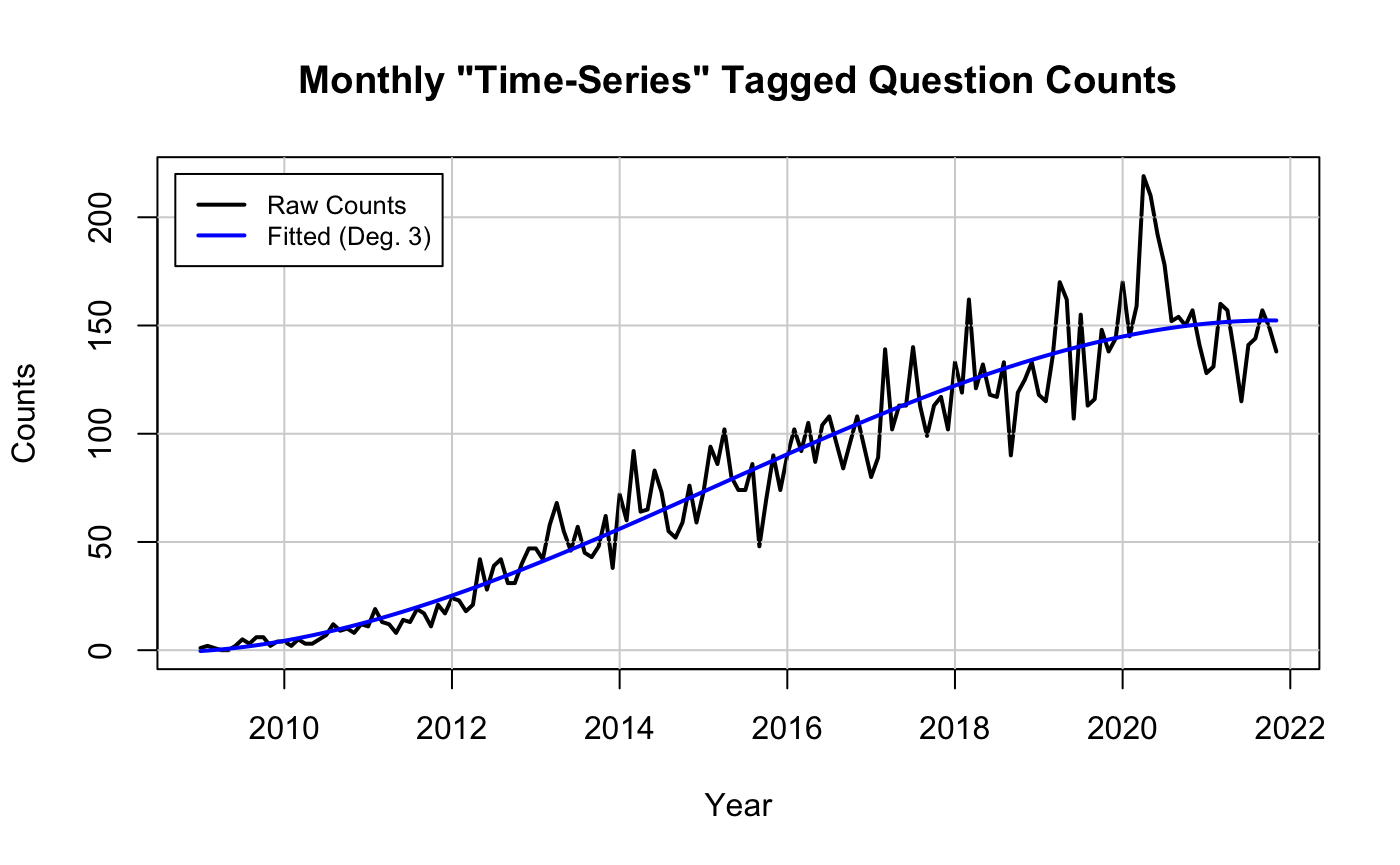
\includegraphics[height=100mm, width=125mm]{deg3_fit_raw_counts.png}
    \caption{Third-Order Polynomial Fit Over Raw Counts}
\end{figure}

\begin{figure}[ht!]
    \centering
    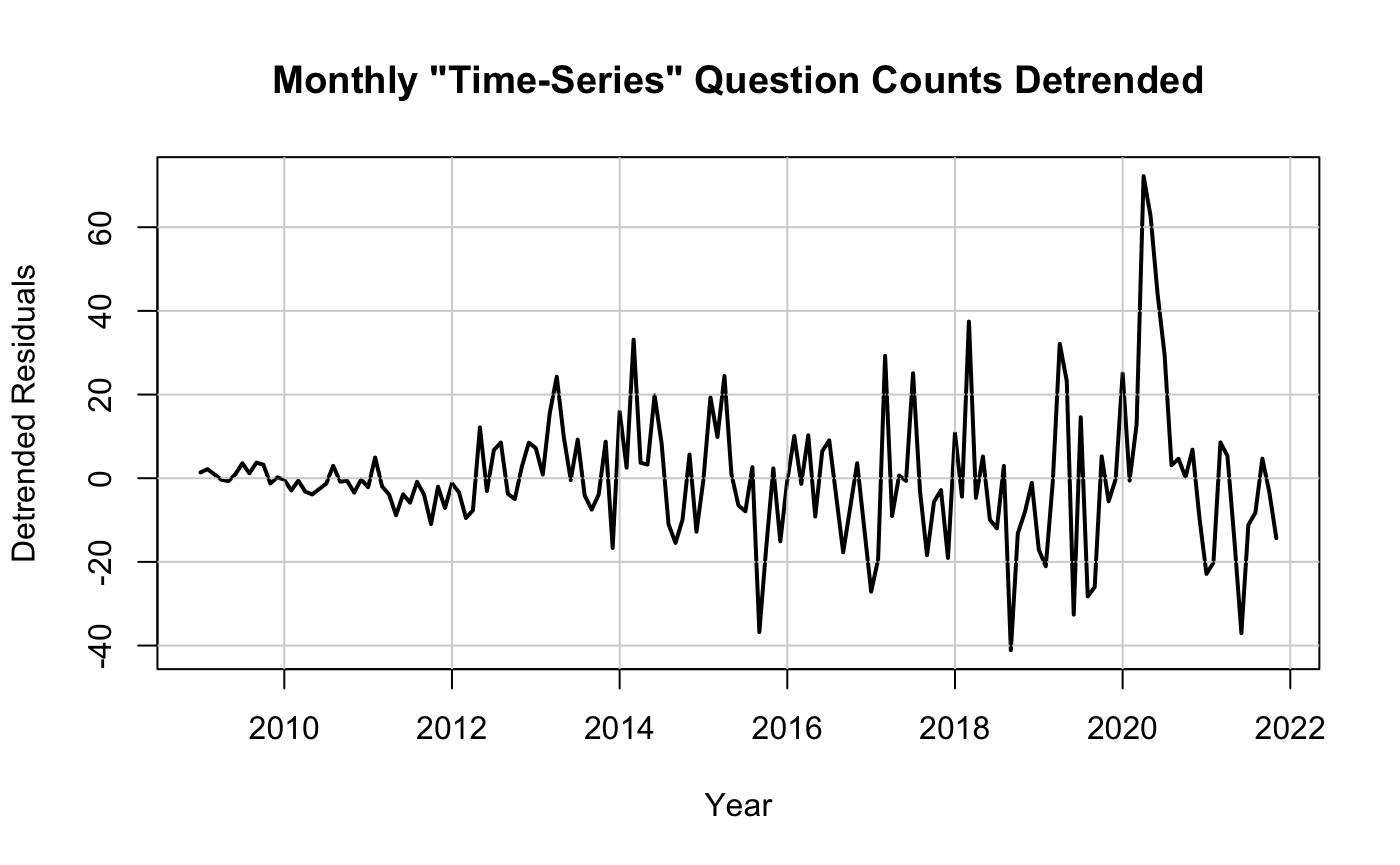
\includegraphics[height=100mm, width=125mm]{detrended_residuals.png}
    \caption{Detrended Residuals (Using Deg. 3 Polynomial for $\hat \mu_t$)}
\end{figure}

\begin{figure}[ht!]
    \centering
    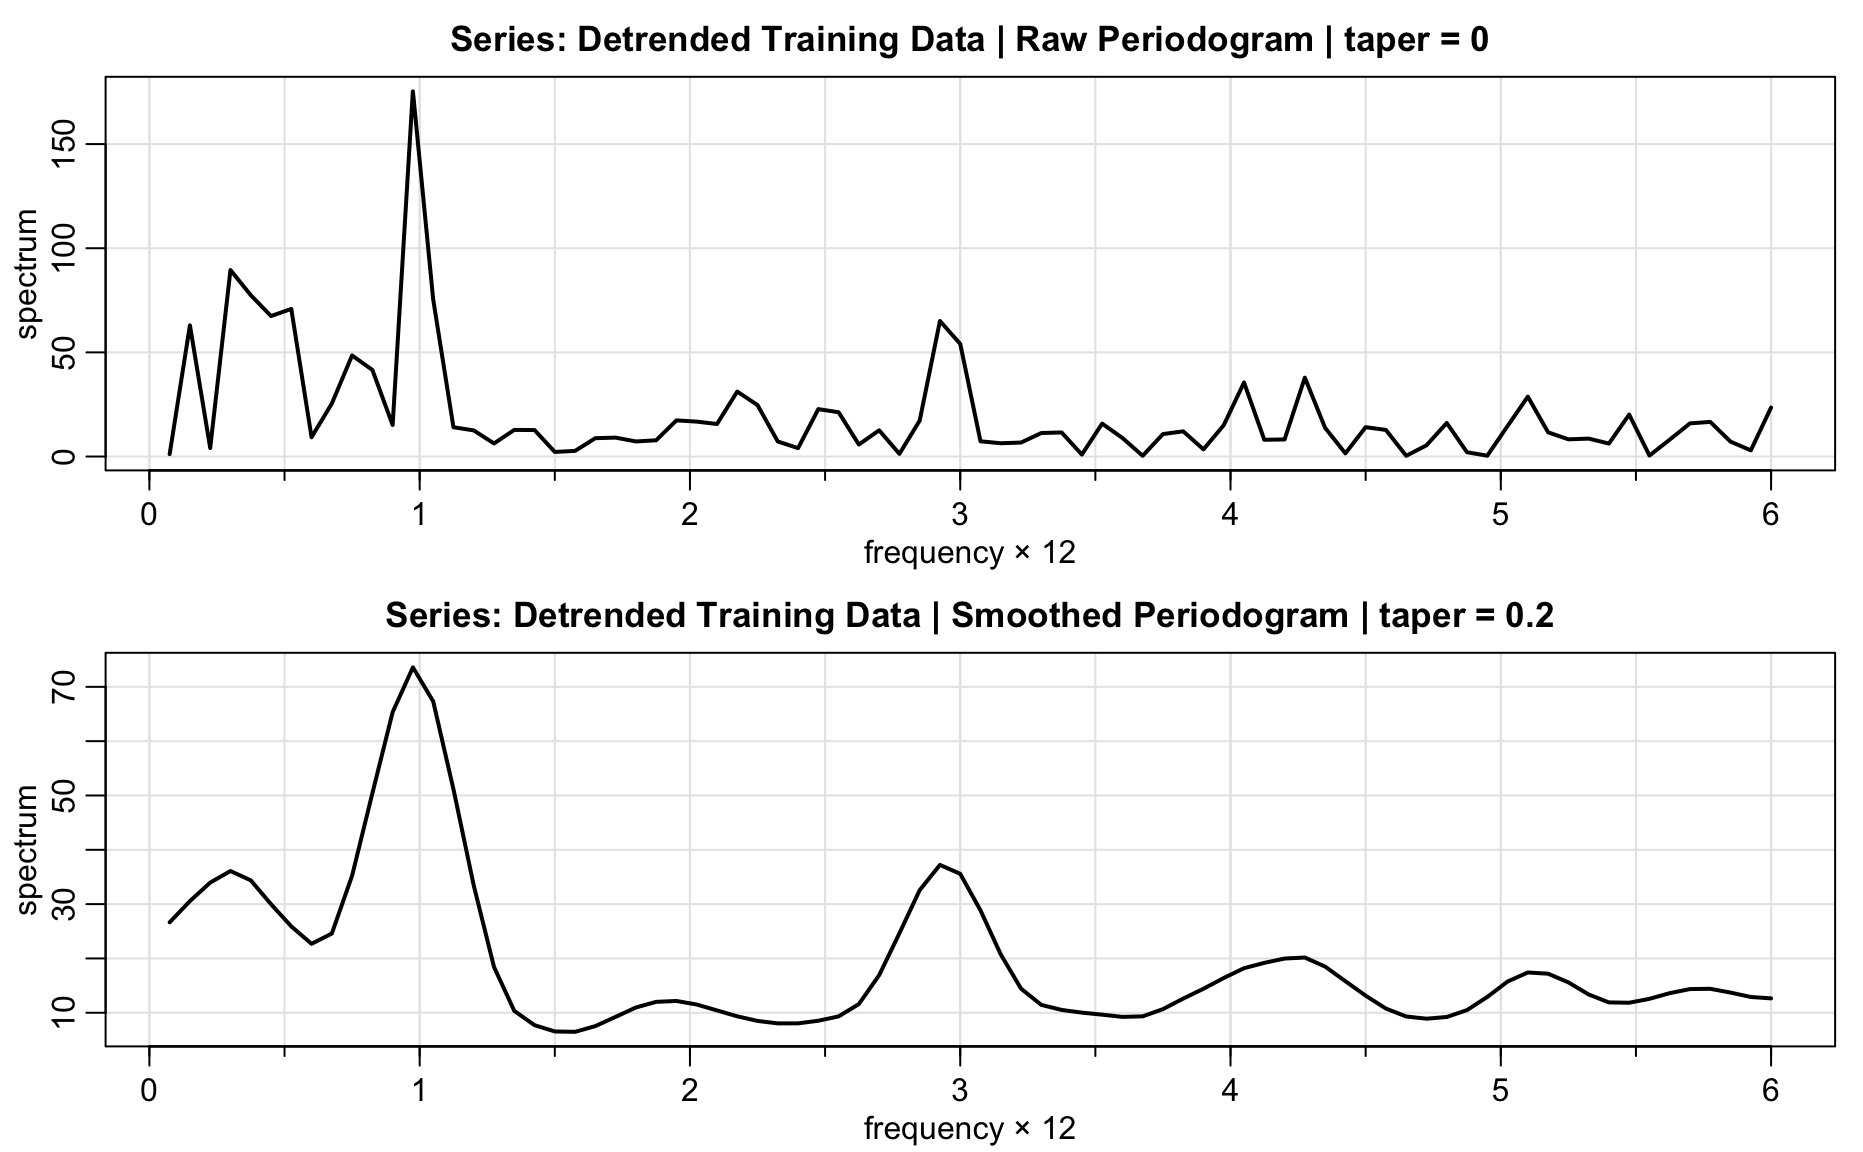
\includegraphics[height=100mm, width=125mm]{nonparam-spec.png}
    \caption{Spectral Estimates for Detrended Residuals}
\end{figure}

\begin{figure}[ht!]
    \centering
    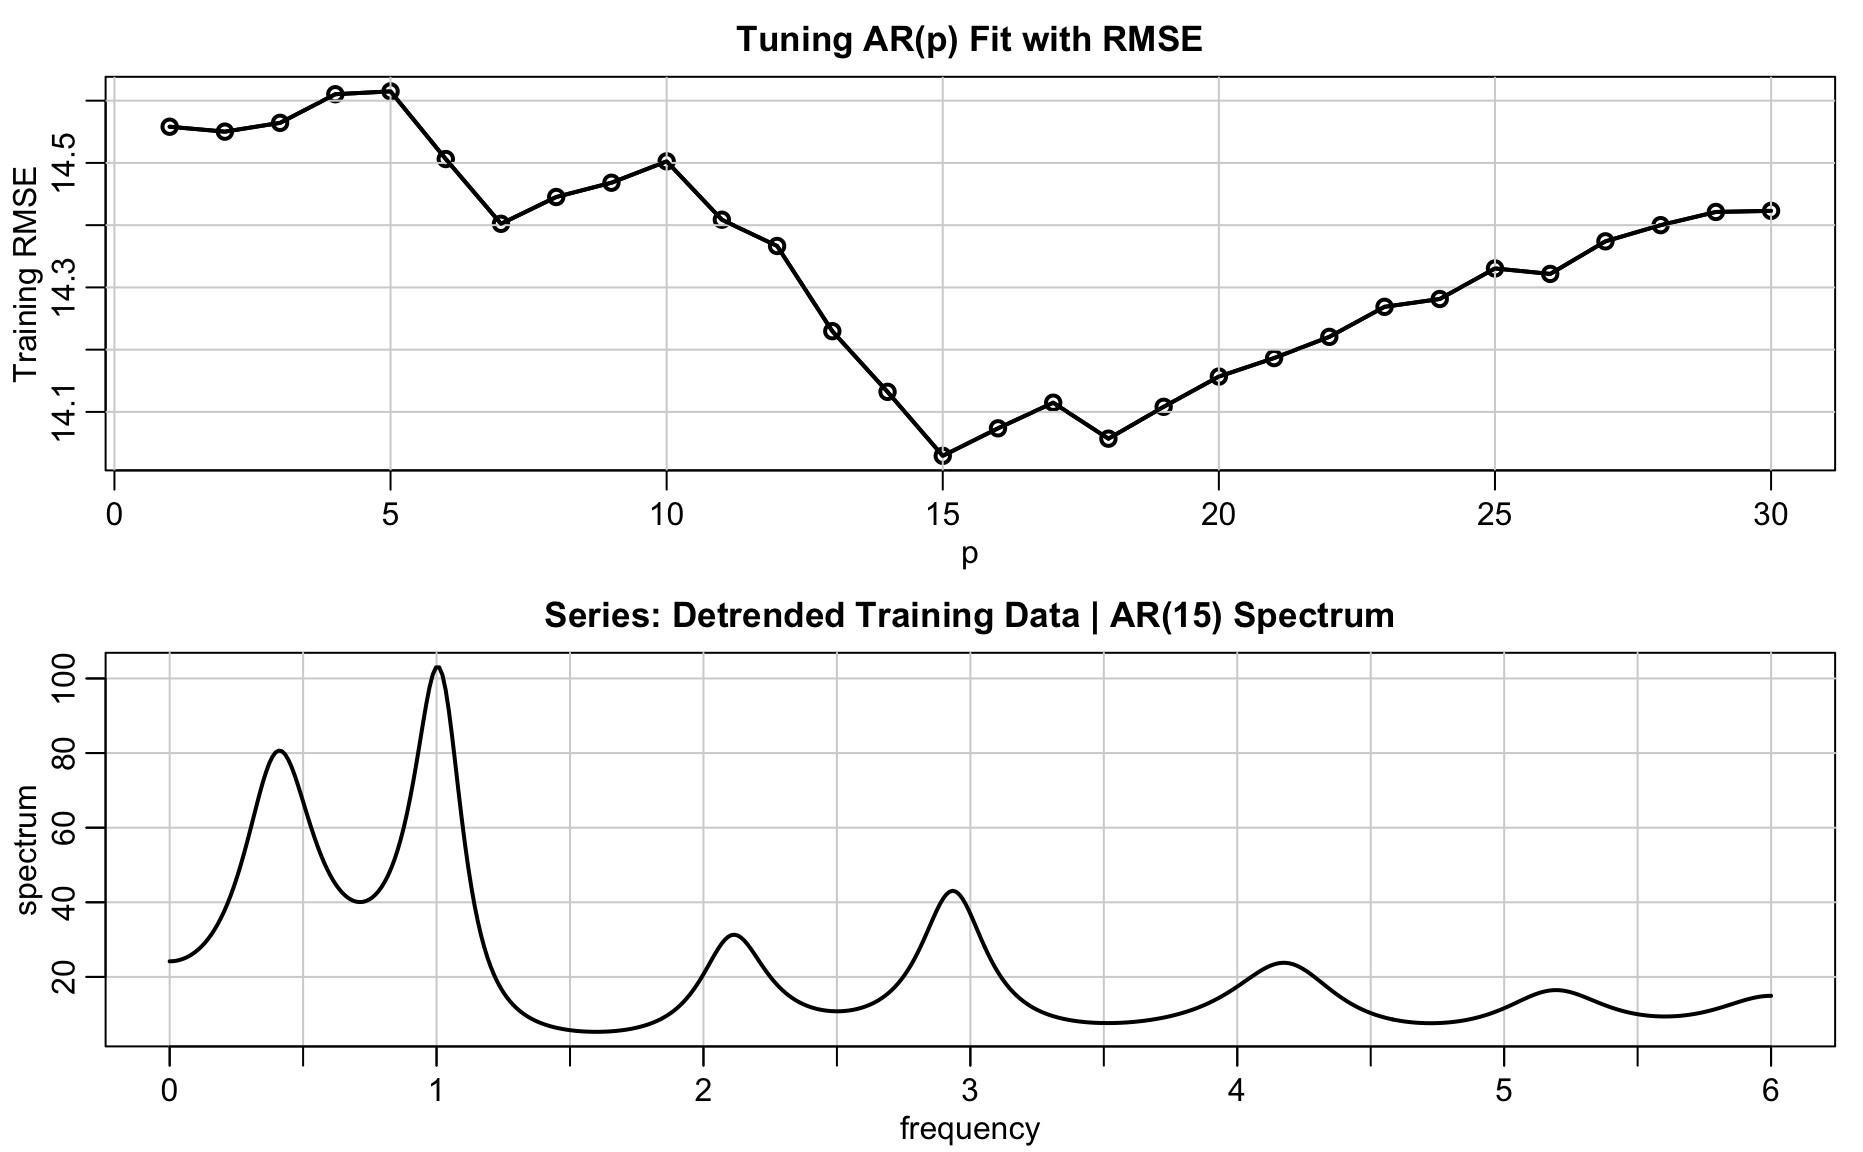
\includegraphics[height=100mm, width=125mm]{tuning-AR-spec.png}
    \caption{AR Spectral Estimation for Detrended Residuals}
\end{figure}

\begin{table}[h!]
    \centering
    \begin{tabular}{| c | c | c | c |} 
    \hline
    95\% C.I. & Freq. $\times$ 12& Lower & Upper \\ 
    \hline
    \hline
    Two-Sided & $\approx$ 0.3 & 18.68 & 96.92\\
    \hline
    Two-Sided & $\approx$ 1 & 38.08 & 197.61\\
    \hline  
    Two-Sided & $\approx$ 3 & 19.26 & 99.95\\
    \hline  
    One-Sided & $\approx$ 0.3 & 20.71 & $\infty$\\
    \hline
    One-Sided & $\approx$ 1 & 42.23 & $\infty$\\
    \hline  
    One-Sided & $\approx$ 3 & 21.36 & $\infty$\\
    \hline  
    \end{tabular}
    \caption{Non-Parametric Spectral Estimation Confidence Intervals}
\end{table}

\begin{figure}[ht!]
    \centering
    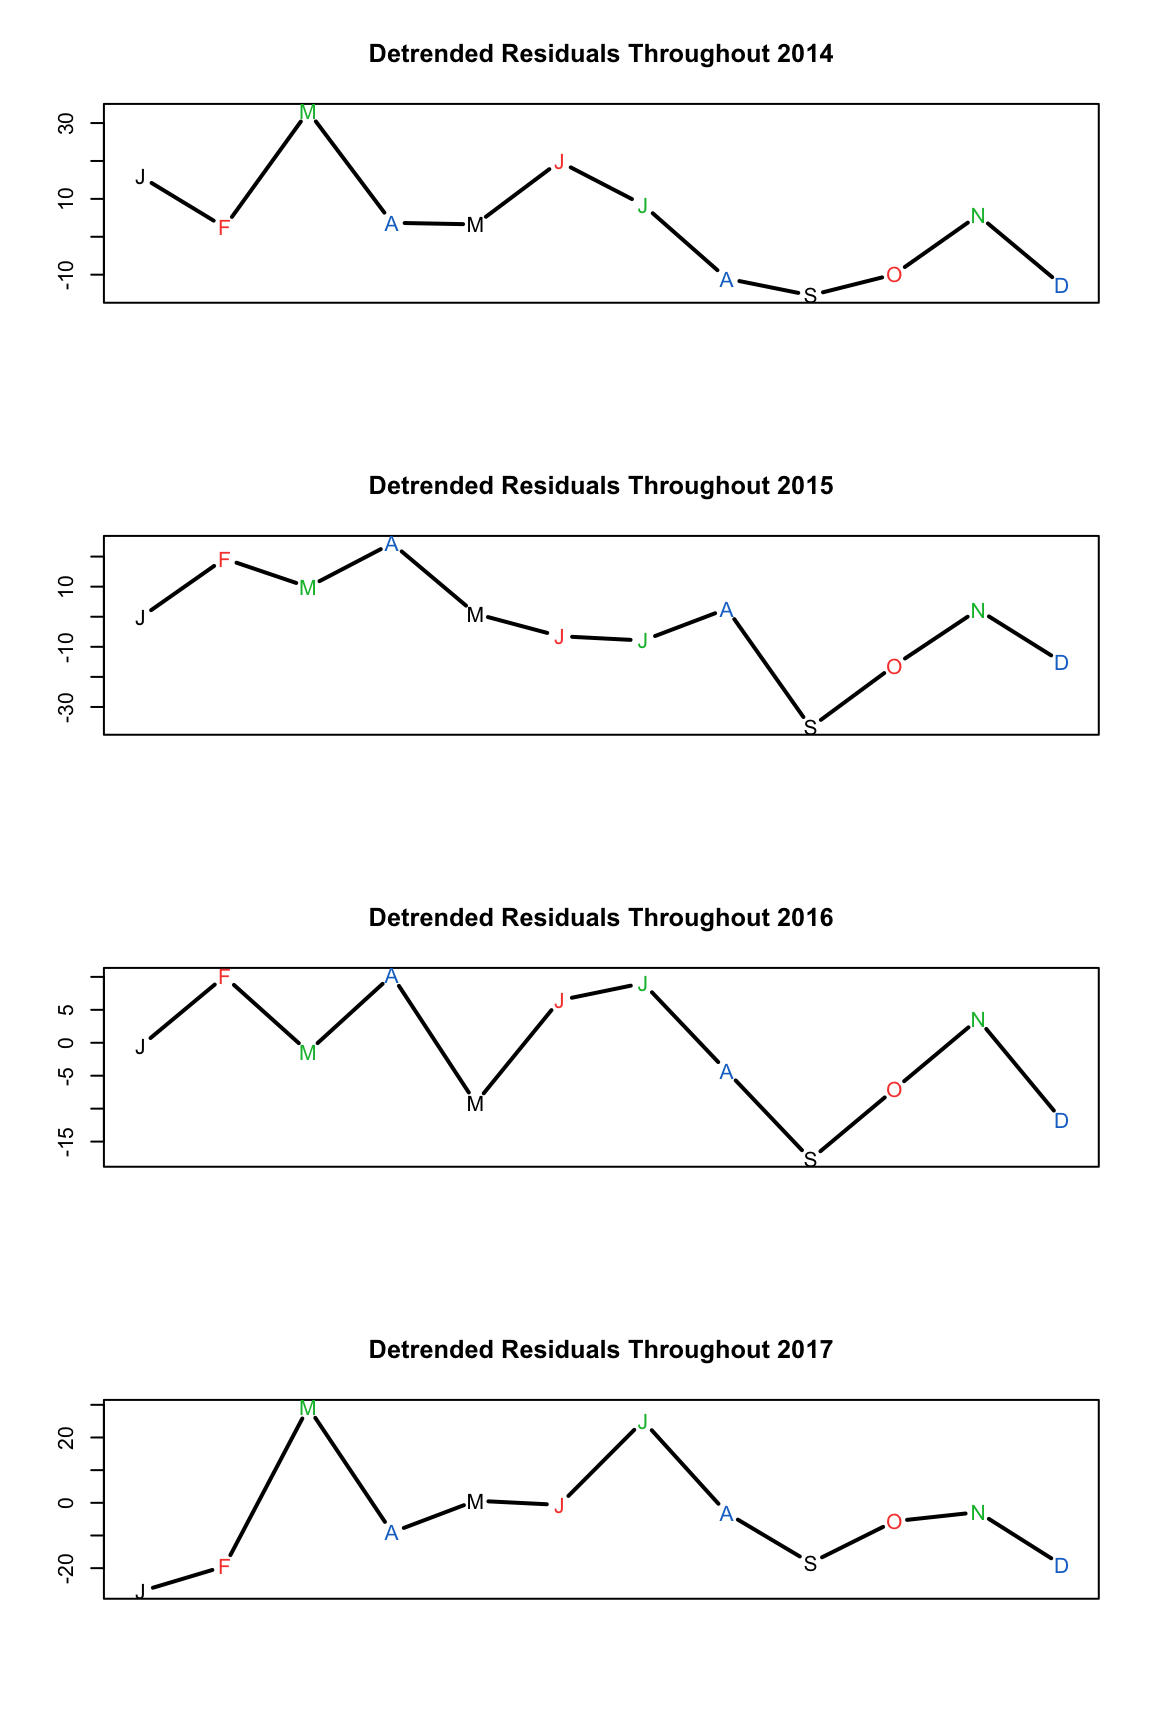
\includegraphics[height=185mm, width=135mm]{annual-cycles.png}
    \caption{Annual Cycles for 2014 to 2017}
\end{figure}

\begin{figure}[ht!]
    \centering
    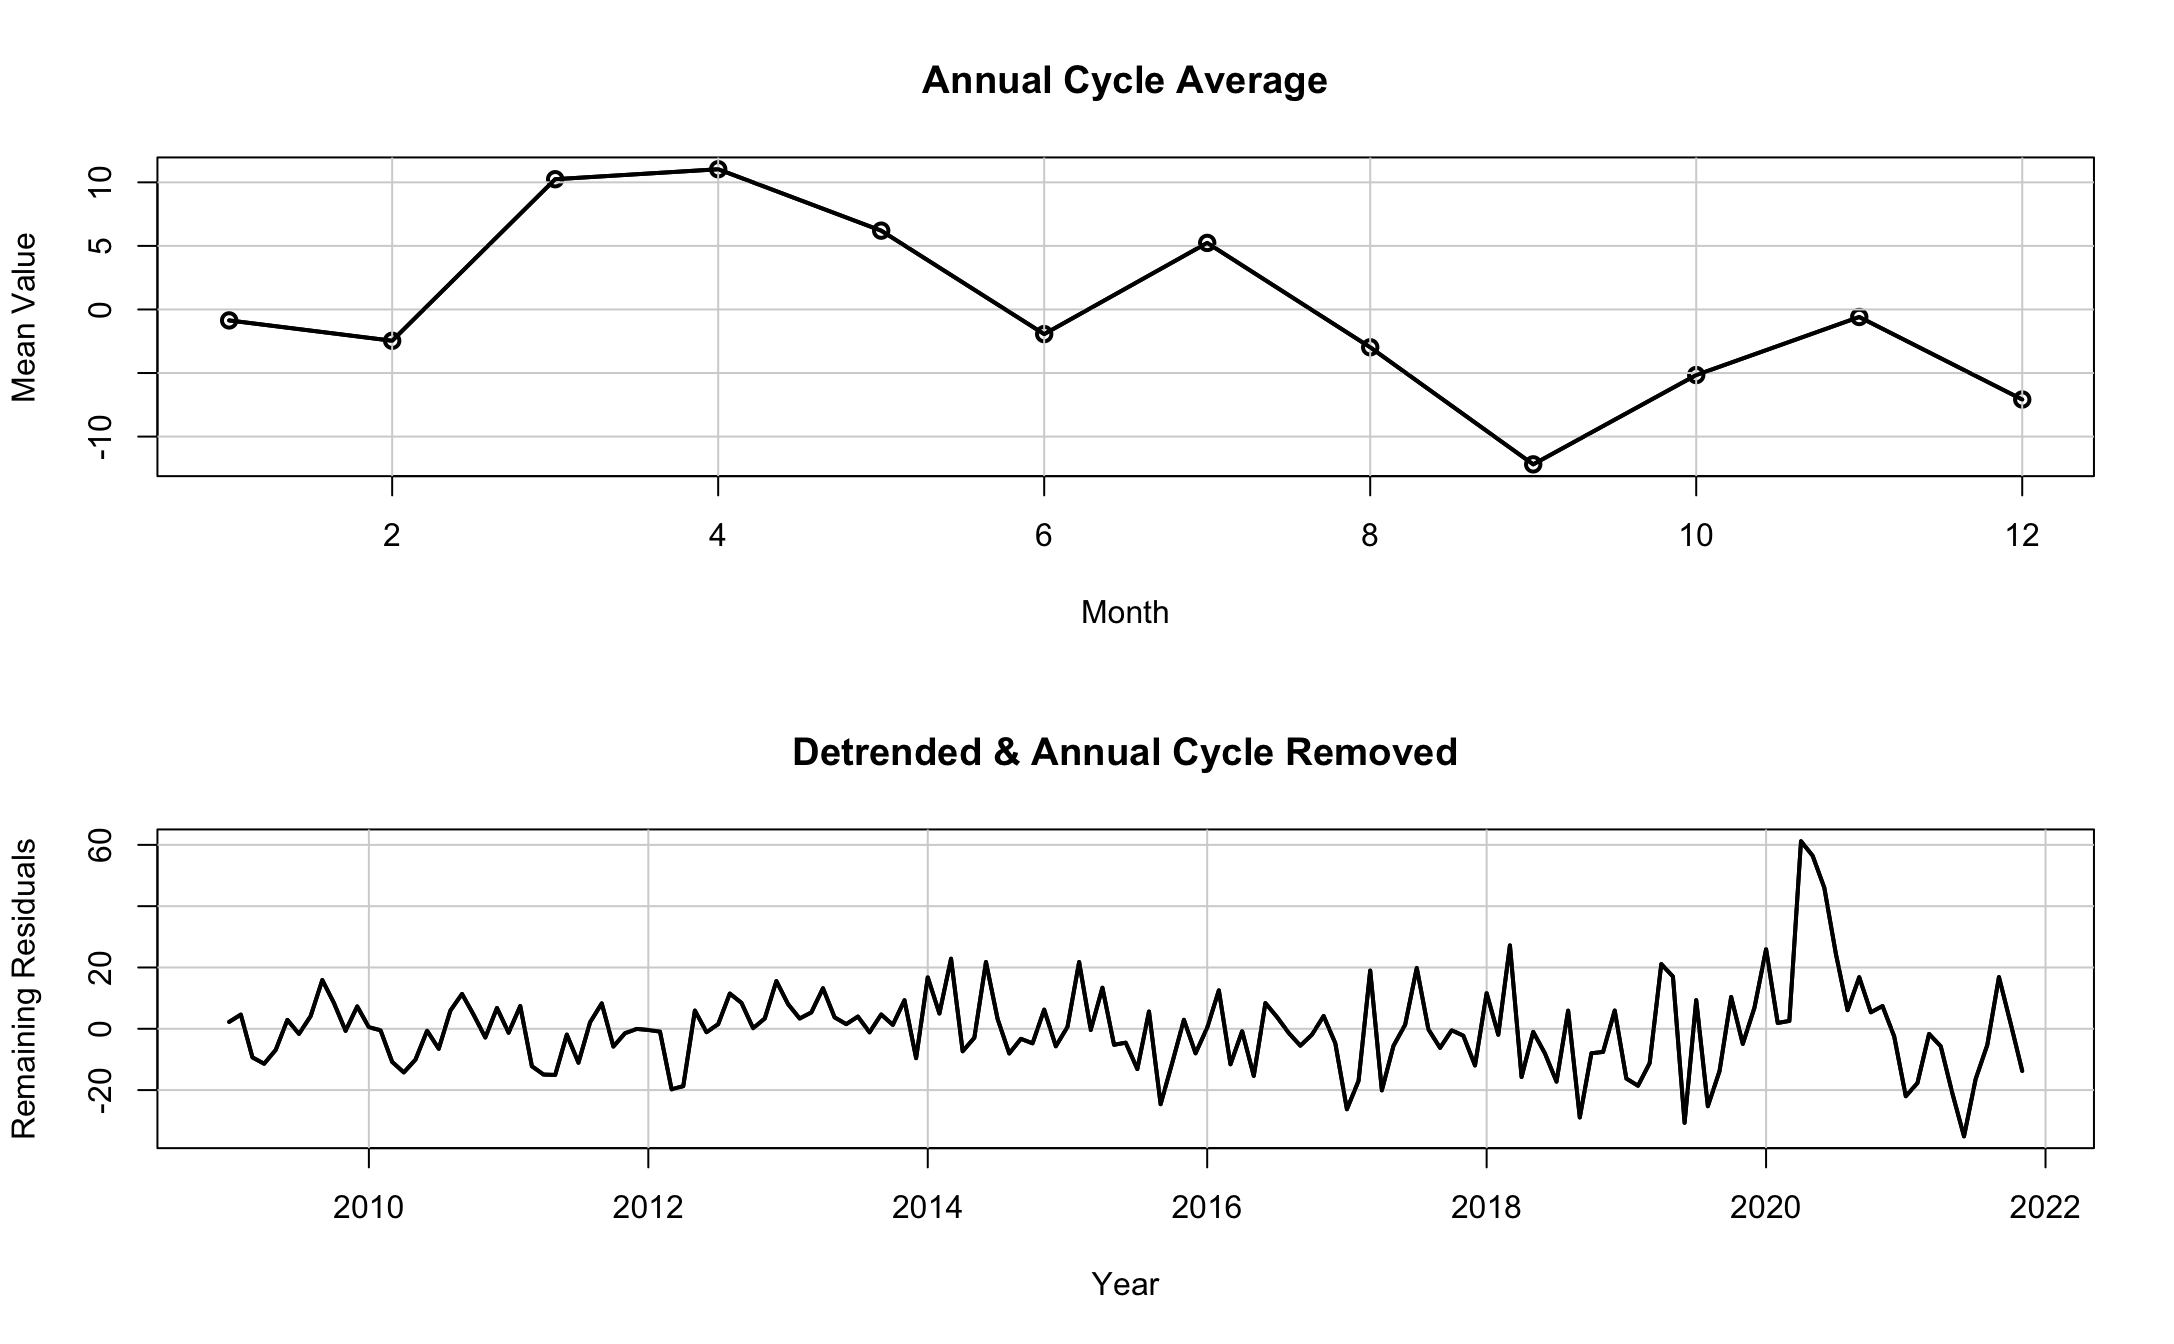
\includegraphics[height=100mm, width=125mm]{annual-cyc-removed.png}
    \caption{Annual Cycle's Average Values (top) \& Remaining Residuals (bottom)}
\end{figure}

\begin{figure}[ht!]
    \centering
    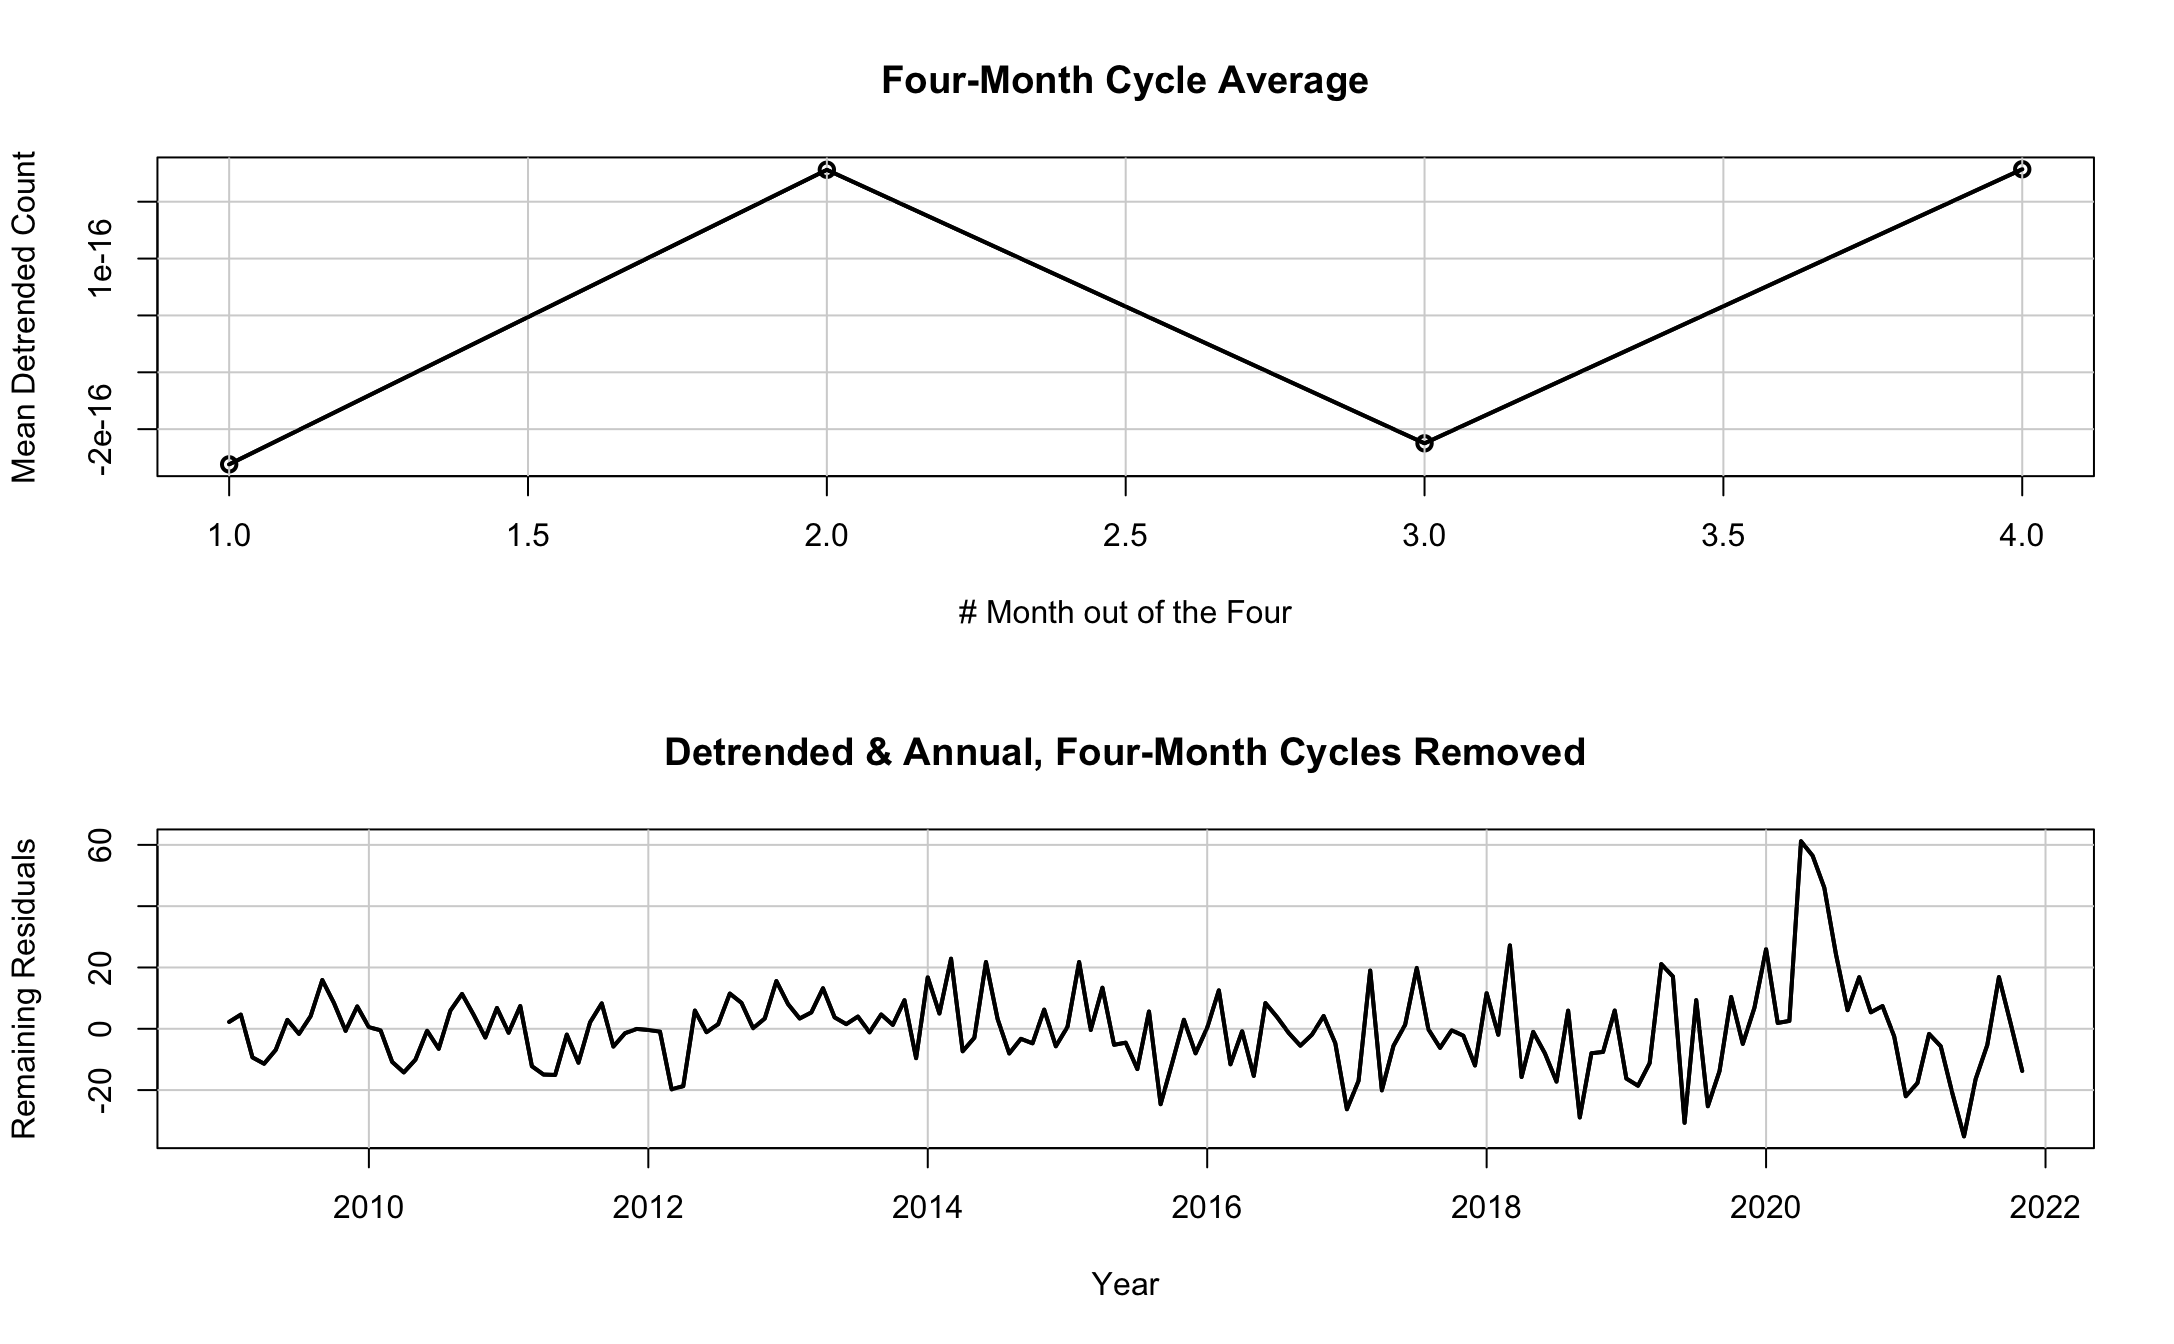
\includegraphics[height=100mm, width=125mm]{4m-cyc-removed.png}
    \caption{Four-month Cycle's Average Values (top) \& Remaining Residuals (bottom)}
\end{figure}

\begin{figure}[ht!]
    \centering
    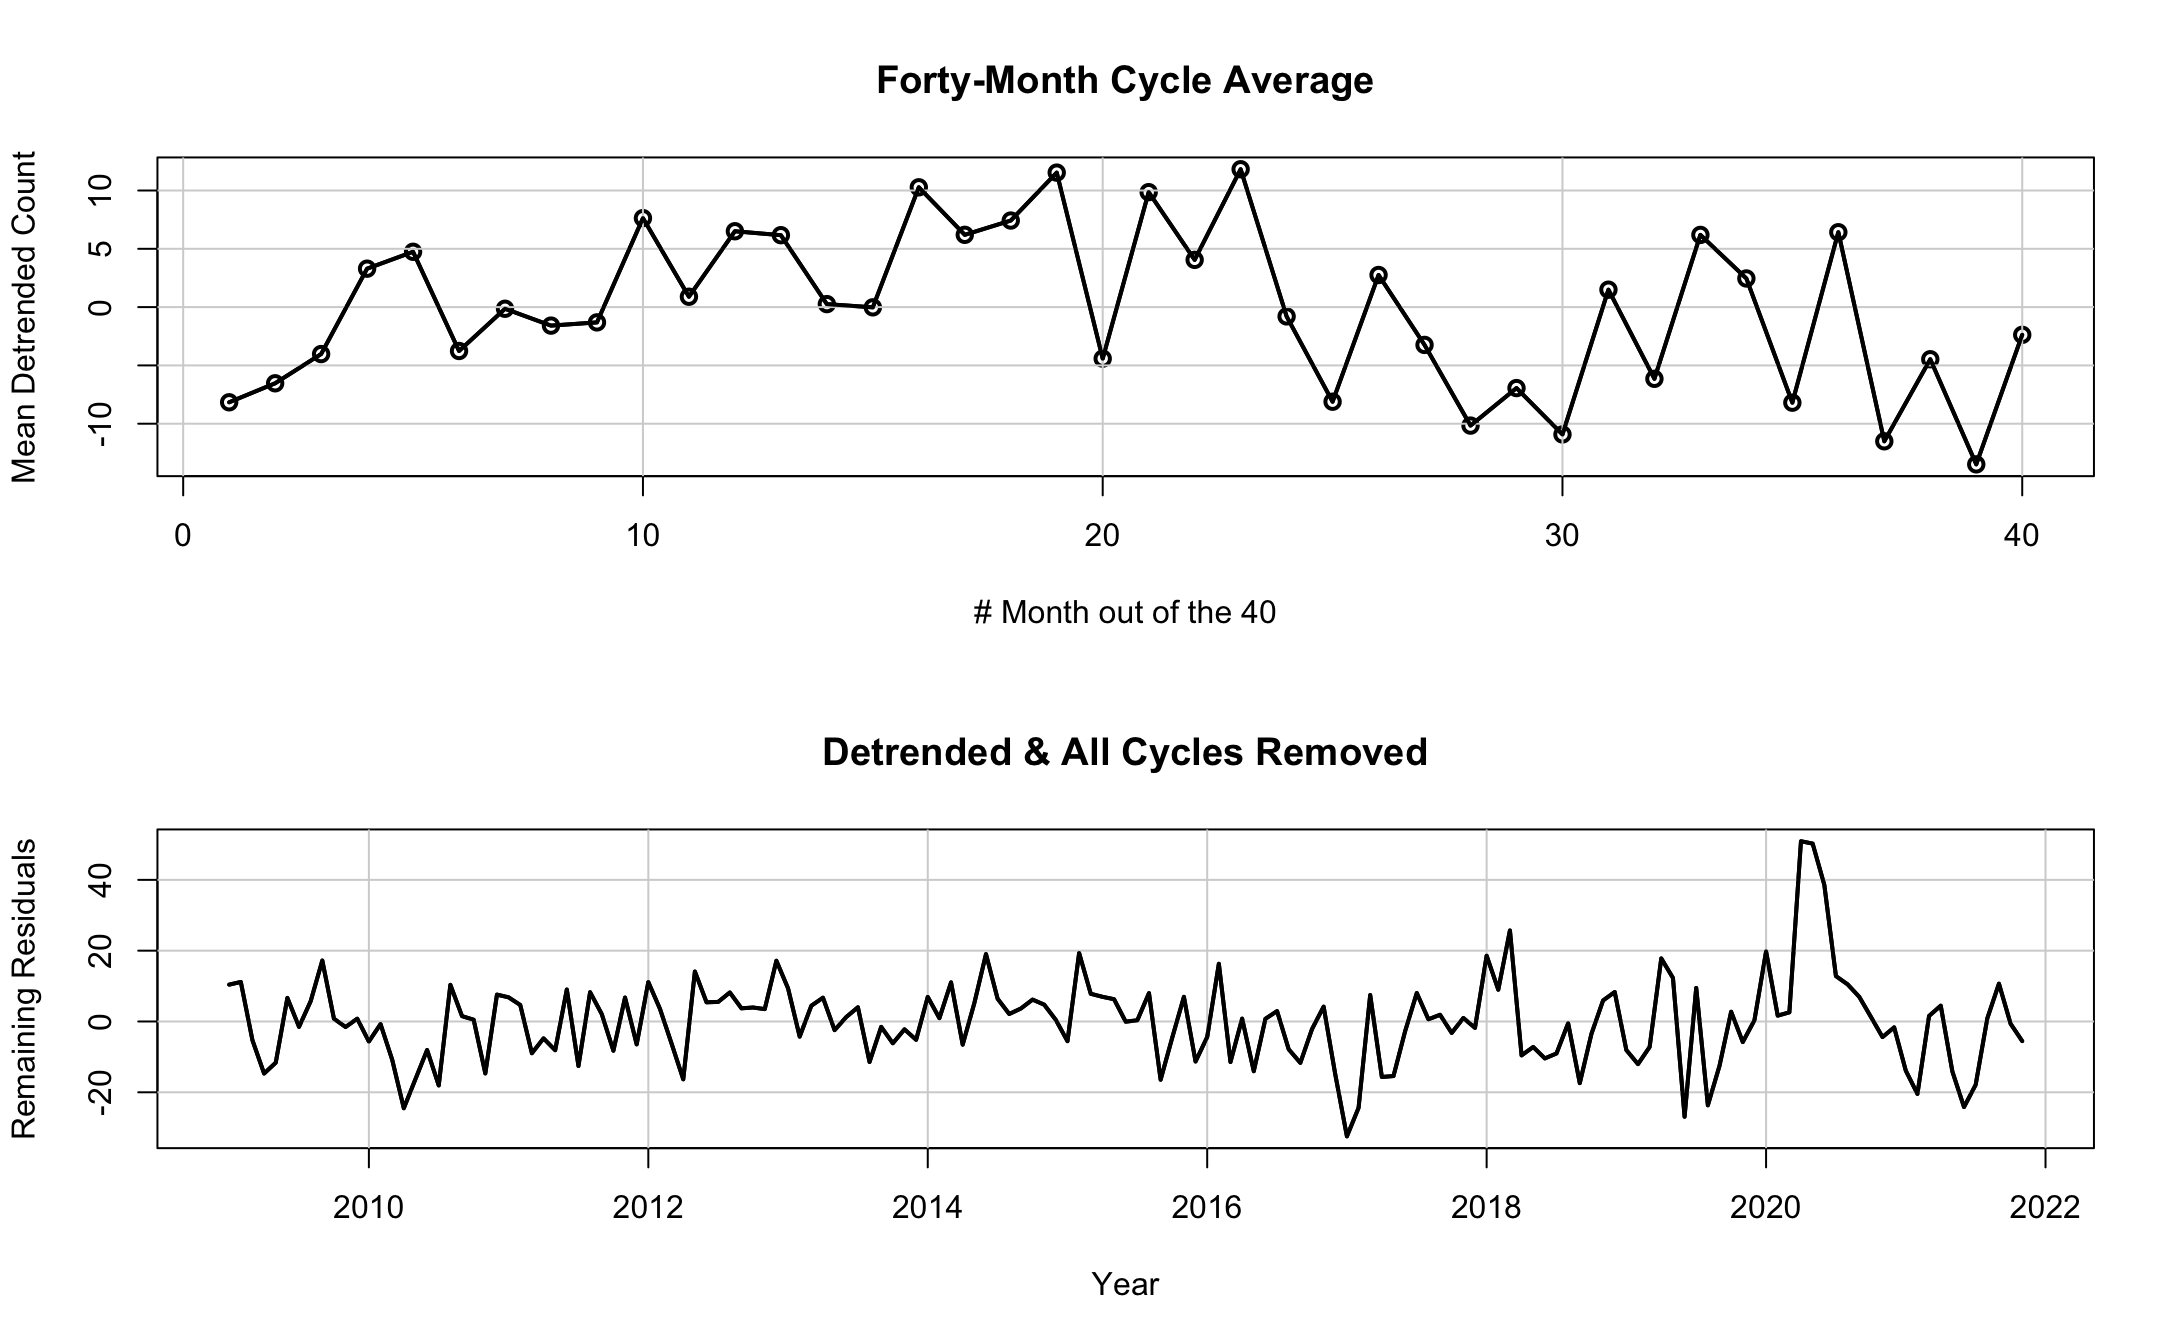
\includegraphics[height=100mm, width=125mm]{40m-cyc-removed.png}
    \caption{Forty-month Cycle's Average Values (top) \& Final Residuals (bottom)}
\end{figure}

\begin{figure}[ht!]
    \centering
    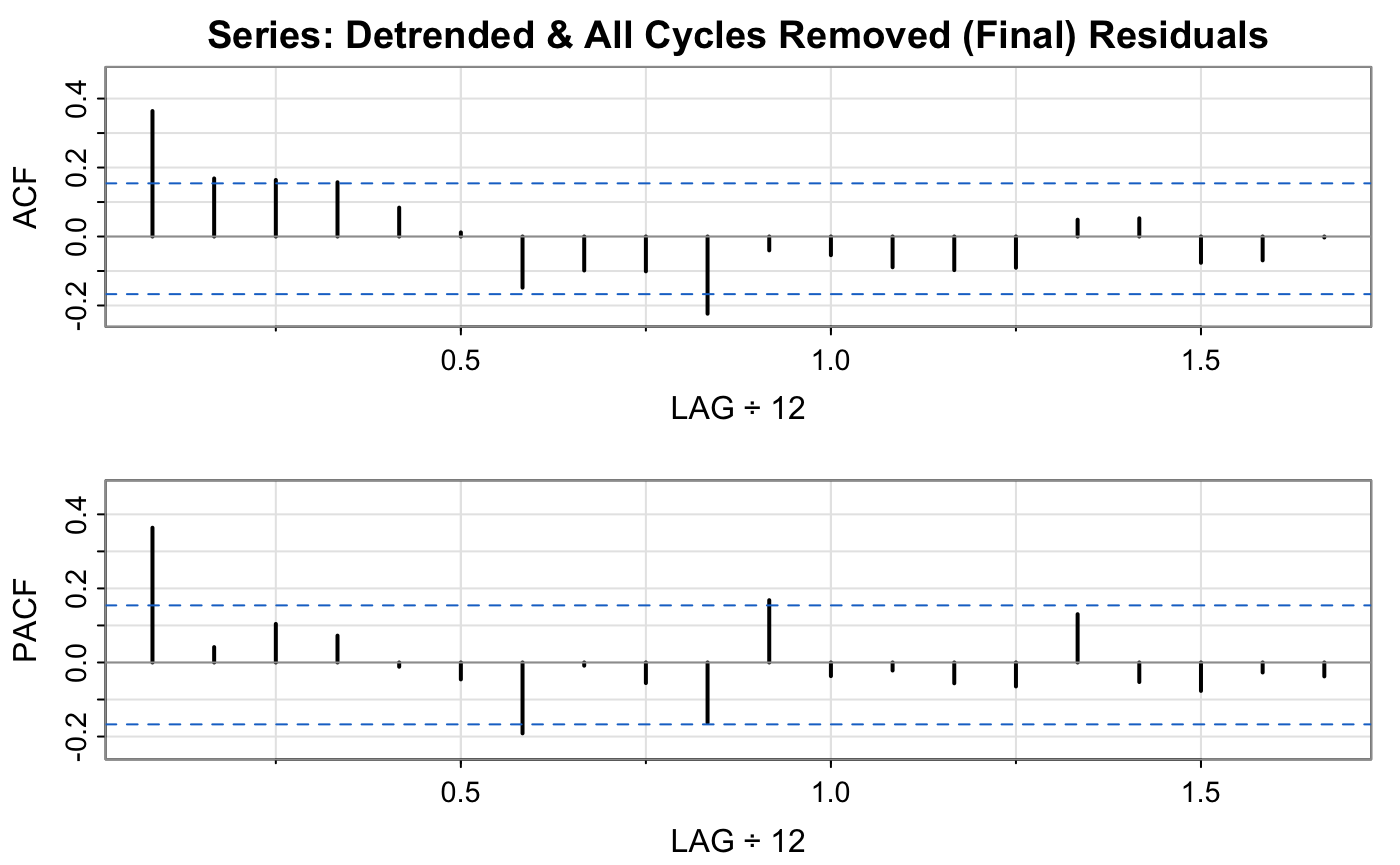
\includegraphics[height=85mm, width=115mm]{acf_pacf_final.png}
    \caption{ACF and PACF of the Detrended and Cycle-Removed Residuals}
\end{figure}

\begin{figure}[ht!]
    \centering
    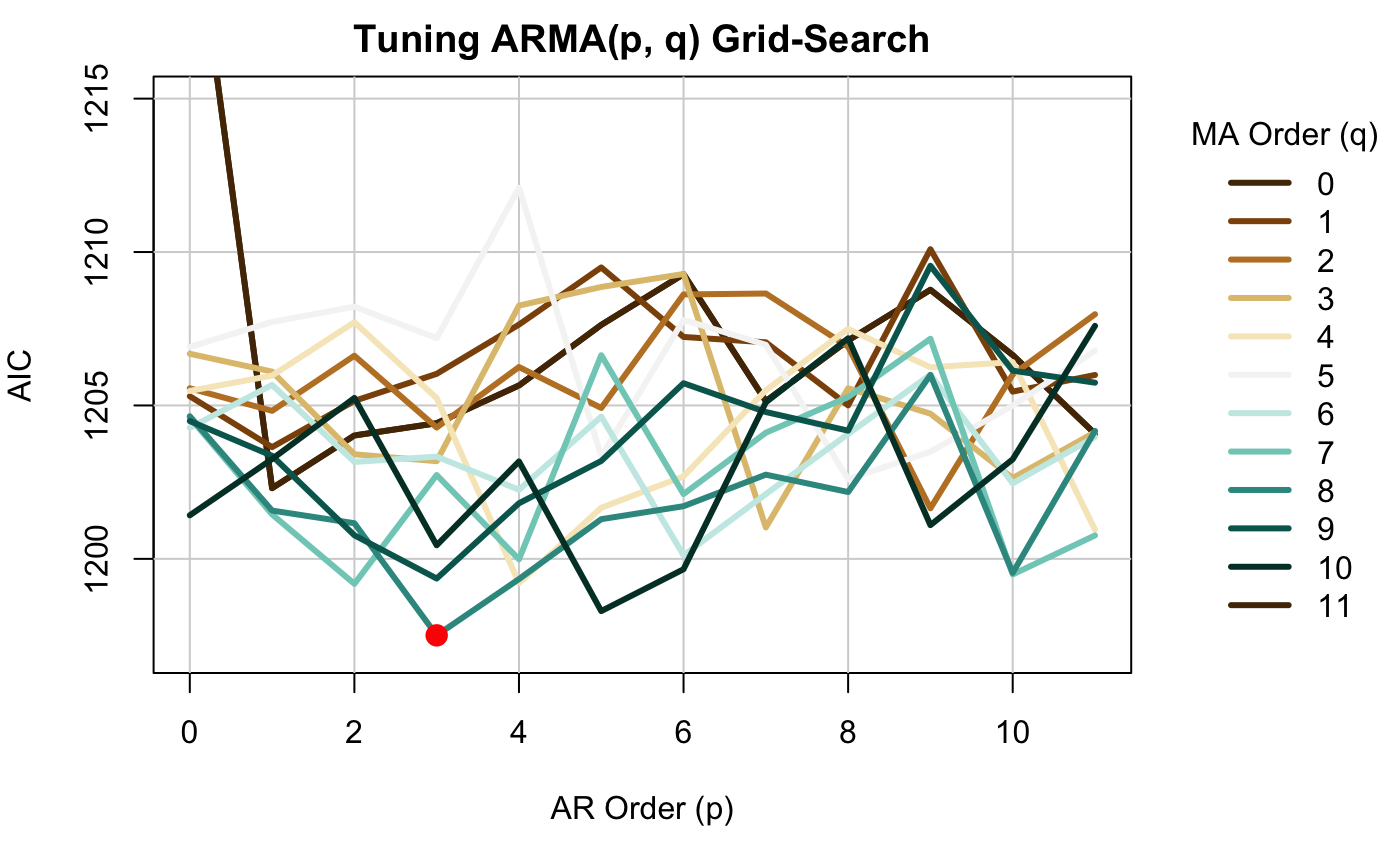
\includegraphics[height=100mm, width=125mm]{tuning.png}
    \caption{AIC Values for Each ARMA($p$, $q$) Model}
\end{figure}

\begin{figure}[ht!]
    \centering
    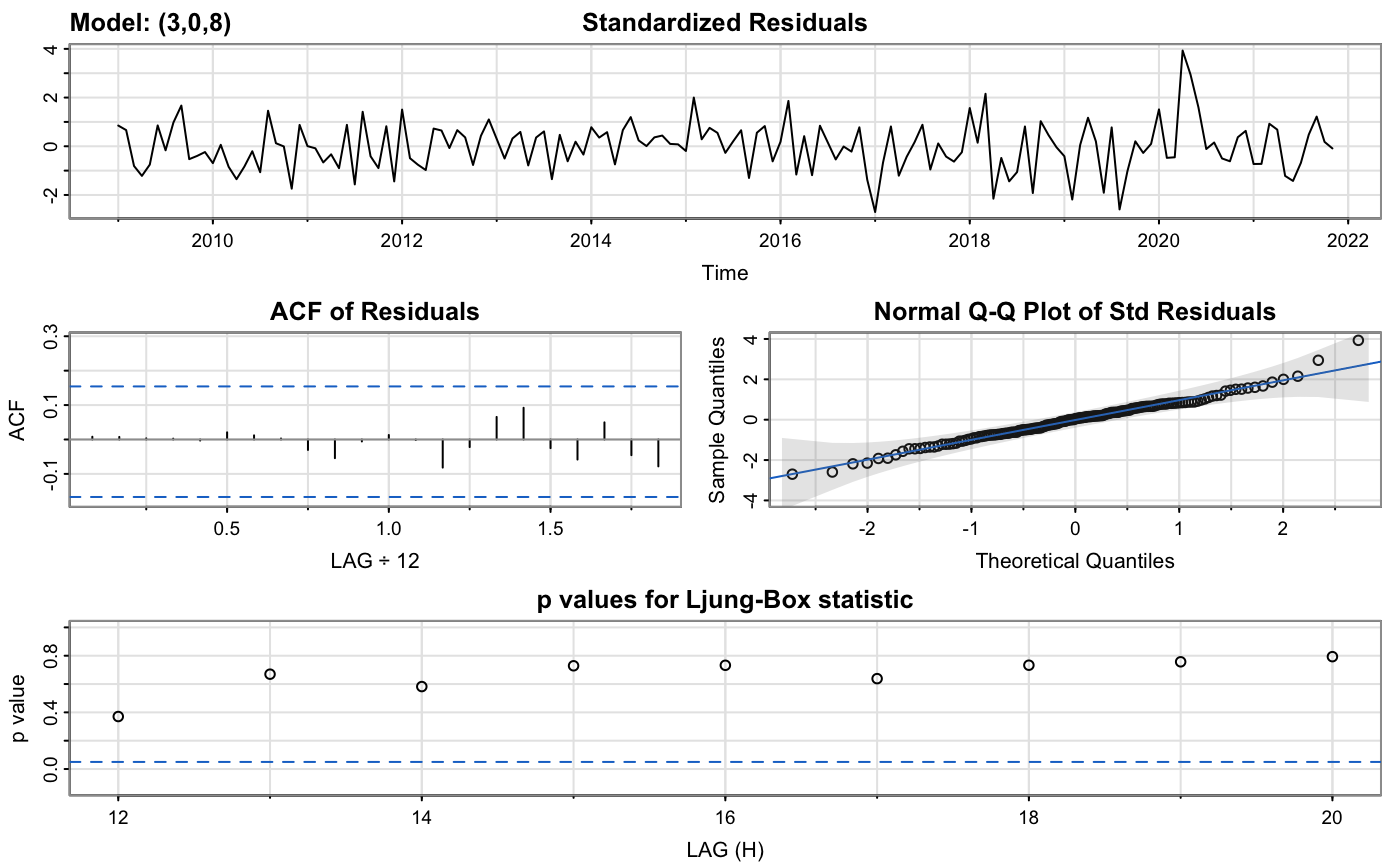
\includegraphics[height=100mm, width=125mm]{diagnostics.png}
    \caption{Diagnostic Plots for Fitted ARMA(3, 8) Model}
\end{figure}

\begin{figure}[ht!]
    \centering
    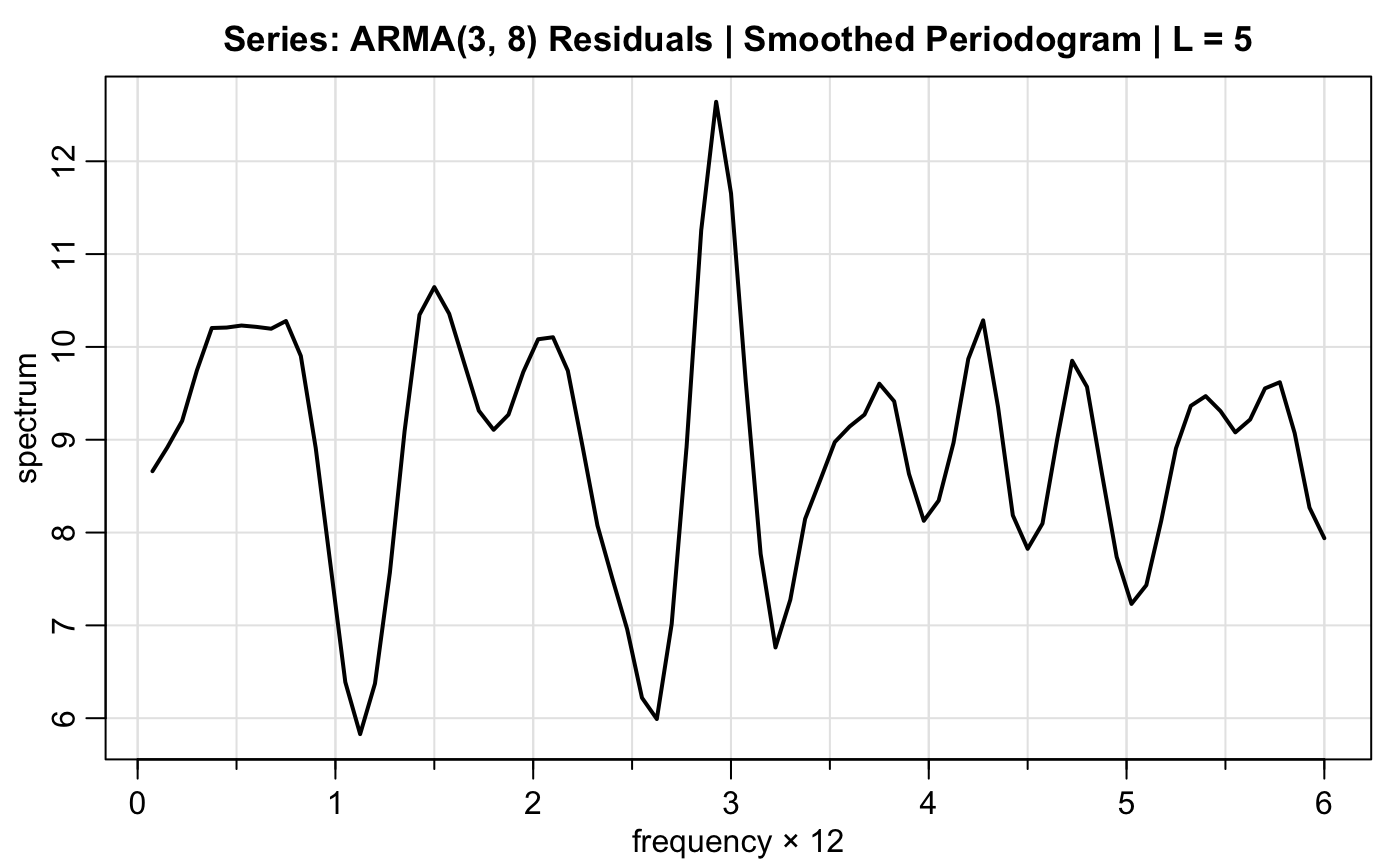
\includegraphics[height=100mm, width=125mm]{arma_res_spec.png}
    \caption{Spectrum for Fitted ARMA(3, 8) Residuals}
\end{figure}

\begin{figure}[ht!]
    \centering
    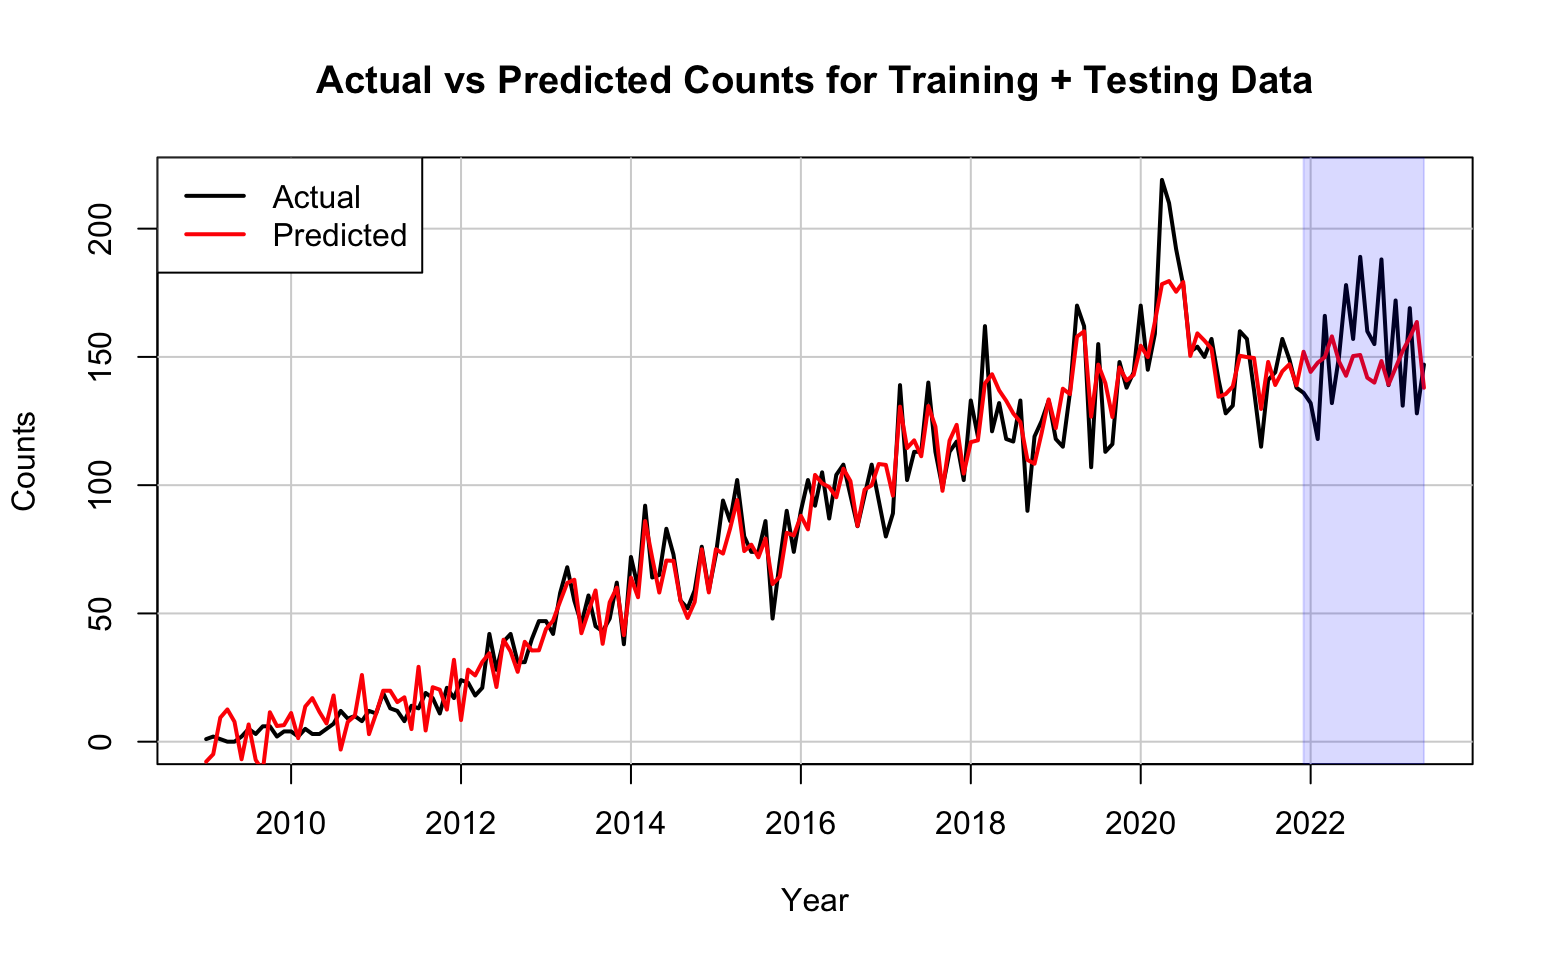
\includegraphics[height=100mm, width=125mm]{pred_counts_overlayed.png}
    \caption{Training and Testing Predictions Over Original Counts}
\end{figure}

\begin{figure}[ht!]
    \centering
    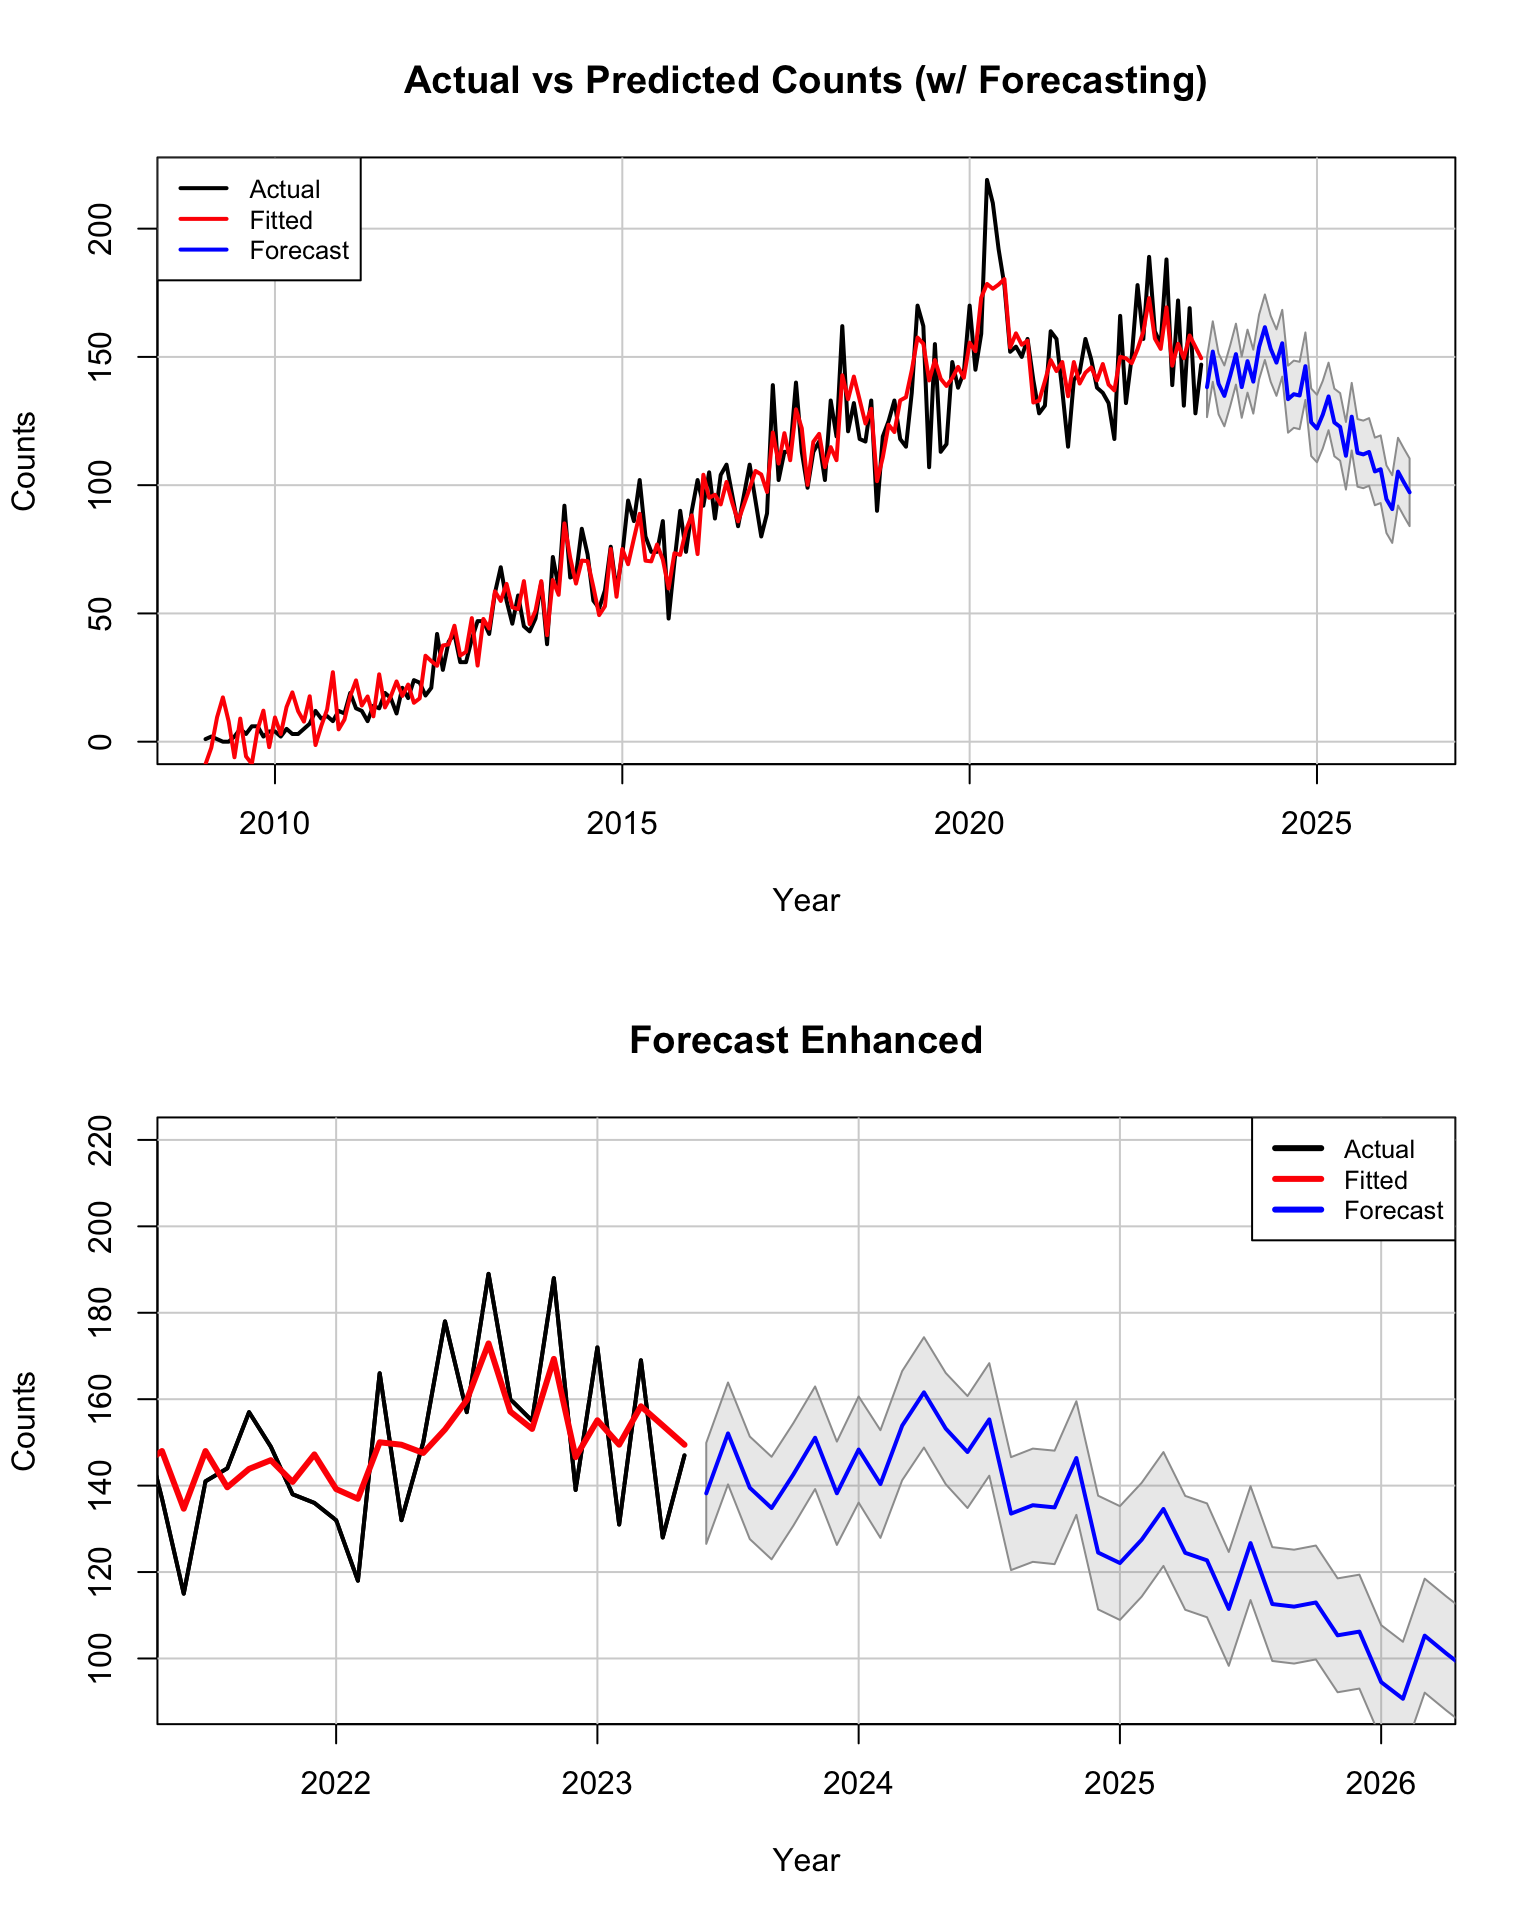
\includegraphics[height=175mm, width=145mm]{forecasting.png}
    \caption{Monthly Counts with Fitted Values and Forecasts}
\end{figure}

\FloatBarrier

\subsection*{Code}

To extract the monthly ``time-series'' related questions from the Stack Exchange Data Explorer, we used the SQL query shown below:

\

\lstinputlisting{code/getSEcounts.sql}

\


We include the R code used for our analysis and modeling below:

\

\lstinputlisting{code/Fc_StackEx_Counts_Code.R}


\end{document}